% \raggedbottom 
\chapter{\uppercase {minor loop constitutive mode*}}
\blfootnote{*Part of this chapter is reprinted with permission from "Nonlinear and time dependent behaviors of piezoelectric materials and structures" by Sohrabi, A., Muliana, A., (2015). \textit{International Journal of Mechanical Sciences}, 94, 1-9,  Copyright 2015 Elsevier Ltd.}
% \chapter[\uppercase {Our cluster value theorems*}]{\uppercase {Our cluster value theorems*}\footnotetext{*Part of this chapter is reprinted with permission from W.~B.~Johnson, S.~Ortega Castillo, \emph{The cluster value problem in spaces of continuous functions}, to appear in Proc.~Amer.~Math.~Soc.}}
% \chapter{\uppercase{minor loop constitutive model}}  
\label{section:minor_loop_constitutive_model_for_polarized_piezo_electric}
This chapter discusses a time-dependent constitutive model for polarized piezoelectric materials with an intention to capture minor hysteretic response.
The model is suitable for piezoelectric ceramics, which experience small deformation gradient, and can sustain large electric fields. 
It is assumed that the loading is within a quasi-static condition so that we neglect the inertia effect on the electro-mechanical response and ignore the energy dissipation effect. 
The constitutive model for a polarized ferroelectric ceramics is obtained from:


\begin{equation}
\begin{aligned}
&\sigma _{ij} = \frac{\partial \Psi_e}{\partial \varepsilon_{ij}}\vert _{E_{k}}
\\
& D_k = -\frac{\partial \Psi_e}{\partial E_k}\vert _{\varepsilon_{ij}}\\
& \Psi_e= \hat{\Psi}_e(E_k,\varepsilon_{ij})
\end{aligned}
\label{EQN:Derivation_from_gibbs}
\end{equation}
where $\hat{\Psi}_e(E_k,\varepsilon_{ij})$ is the thermodynamics function expressed in terms of the electric field vector $E_k$ and strain tensor $\varepsilon_{ij}$. 
The notations $\vert _{E_{k}}$ and $\vert _{\varepsilon_{ij}}$ mean that the field variables are evaluated at constant $E_{k}$ and $\varepsilon_{ij}$, respectively.
The thermodynamics potentials are often expressed in a Taylor series expansion of the independent field variables that can include higher order terms. 
Following the constitutive model of Tiersten \cite{tiersten1993electroelastic}
for active materials undergoing large electric fields and small strains, 
the free energy $\hat{\Psi}_e(E_k,\varepsilon_{ij})$ at an isothermal condition is then expressed as:

\begin{equation}
\begin{aligned}
&\hat{\Psi}_e=
\sum_{i,j,k,l=1}^{3} \frac{1}{2}C_{ijkl}{\varepsilon _{ij}}{\varepsilon _{kl}}-
\sum_{k,i,j=1}^3 e_{kij}\varepsilon _{ij}E_k-
\sum_{k,j=1}^3 \frac{1}{2}\kappa _{kj}{E_j}{E_k}-\\
&
\sum_{i,j,k,l=1}^3 \frac{1}{2}\hat{b}_{klij}{E_k}{E_l}\varepsilon _{ij}+
\sum_{i,j,k,l=1}^3 \frac{1}{6}\chi_{kij}{E_i}{E_j}{E_k}+H.O.T
\end{aligned}
\label{EQN:Gibbs_Free_Energy}
\end{equation}
where $C_{ijkl}$ are the components of the elastic stiffness, $e_{kij}$ represents the components of electro mechanical coupling tensor and $\kappa _{kj}$ are the components of the electric permittivity tensor. The field variables are the stress $\sigma _{ij}$, strain $\varepsilon _{kl}$, electric displacement $D_k$, and electric field $E_j$.
Moreover, $\hat{b}_{klij}$ and $\chi_{kij}$ are the components of the fourth-order electro-mechanical tensor and third-order electric permeability tensor, respectively. 
Equation  (\ref{EQN:Gibbs_Free_Energy}) can be further expanded to include fourth, fifth, etc. order terms of electric field.
In such case, additional material paramaters are required.
It is also possible to consider only the odd or even terms of electric field in order to capture response of the material.
Using equations  (\ref{EQN:Gibbs_Free_Energy}) and (\ref{EQN:Derivation_from_gibbs}) the stress and electric displacement for piezoelectric materials undergoing small strain and large electric field are written as:
\\
 
\begin{equation}
\begin{aligned}
&\sigma _{ij} = 
\sum_{k,l=1}^3 {C_{ijkl}}{\varepsilon _{kl}} - 
\sum_{k=1}^3 e_{kij}{E_k} -
\sum_{k,l=1}^3 \frac{1}{2}\hat{b}_{ijkl}{E_k}{E_l}\\
&{D_k} =  
\sum_{i,j=1}^3 {e_{kij}}{\varepsilon _{ij}} + 
\sum_{j=1}^3 {\kappa _{kj}}{E_j}+
\sum_{i,j,l=1}^3 \hat{b}_{klij}{E_l}\varepsilon _{ij}+
\frac{1}{2} 
\sum_{i,j=1}^3 \chi_{kij}{E_i}{E_j} \\
& (i,j,k=1 \dots 3)  
\end{aligned}
\label{EQN:Non_Linear_Constitutive_Relation}
\end{equation}

When the nonlinear terms are neglected, a linear electro-mechanical response of piezoelectric material \cite{Leo2007} is then obtained:

\begin{equation}
\begin{aligned}
&\sigma _{ij} = 
\sum_{k,l=1}^3 {C_{ijkl}}{\varepsilon _{kl}} - 
\sum_{k=1}^3 {e_{kij}}{E_k}\\
&{D_k} = 
\sum_{i,j=1}^3 e_{kij}\varepsilon _{ij} + 
\sum_{j=1}^3 \kappa _{kj}{E_j}\\
& (i,j,k=1 \dots 3)
\end{aligned}
\label{EQN:Standanrd_Constitutive_Relation}
\end{equation}

In the above expression, strains and electric fields are chosen as the independent field variables. 
In case of a finite element analysis, displacements $u_i$ and electric potential $\Phi$ are defined at nodes within finite elements. 
The field variables in the constitutive equations are obtained directly from the displacements $u_i$ and electric potential $\Phi$. 
The strain displacement relationship based on infinitesimal strain theory is defined as:

\begin{equation}
\varepsilon_{kl}=\frac{u_{k,l}+u_{l,k}}{2}
\label{EQN:Linear_Displacement}
\end{equation}
where subscript with comma ($_{,l}$) means derivative with respect to $x_l$ ($\frac{\partial}{\partial x_l}$). 
The electric field is defined as:

\begin{equation}
E_j=-\Phi_{,j}
\label{EQN:Linear_Electric_Field}
\end{equation}

For a linear electro mechanical response given in equation
(\ref{EQN:Standanrd_Constitutive_Relation}) the derivatives of the stress and
electric displacement with respect to the independent field variabless result in
the following material parameters:

\begin{equation}
\begin{aligned}
&\frac{\partial \sigma_{ij}}{\partial \varepsilon_{kl}}=C_{ijkl} \\
&\frac{\partial \sigma_{ij}}{\partial E_{k}}=-e_{kij} \\
&\frac{\partial D_{k}}{\partial\varepsilon_{ij}}=e_{kij} \\
&\frac{\partial D_{k}}{\partial E_{i}}=\kappa_{ki}
\end{aligned}
\label{EQN:Linear_Constants}
\end{equation}

For the nonlinear electro-mechanical model such as in equation (\ref{EQN:Non_Linear_Constitutive_Relation}),
the derivatives of the stress and electric displacament with respect to the independent field variables are:

\begin{equation}
\begin{aligned}
&\frac{\partial \sigma_{ij}}{\partial \varepsilon_{kl}}=C_{ijkl} \\
&\frac{\partial \sigma_{ij}}{\partial E_{k}}=
-e_{kij}-
\sum_{l=1}^3 \hat{b}_{klij} E_l\\
&\frac{\partial D_{k}}{\partial \varepsilon_{ij}}=
e_{kij}+
\sum_{l=1}^3 \hat{b}_{klij} E_l \\
&\frac{\partial D_{k}}{\partial E_{i}}=
\kappa_{ki}+
\sum_{m,n=1}^3 \hat{b}_{kimn}\varepsilon _{mn}+
\sum_{j=1}^3 \chi_{kij} E_j\\
\end{aligned}
\label{EQN:Non_LinearLinear_Constants}
\end{equation}

Tiersten \cite{tiersten1993electroelastic} also discussed an alternative expression of the constitutive model with nonlinear electric field and small strain when stress and 
 electric field are taken as the independent field variables

\begin{equation}
\begin{aligned}
&\varepsilon _{ij} = 
\sum_{k,l=1}^3 {S_{ijkl}}{\sigma_{kl}} + 
\sum_{k=1}^3 d_{kij}{E_k} +
\sum_{k,l=1}^3 \frac{1}{2}{f}_{ijkl}{E_k}{E_l}\\
&{D_k} =  
\sum_{i,j=1}^3 {d_{kij}}{\sigma_{ij}} + 
\sum_{j=1}^3 {\kappa^{\sigma}_{kj}}{E_j}+
\sum_{i,j,l=1}^3 {f}_{klij}{E_l} \sigma _{ij}+\frac{1}{2} 
\sum_{i,j=1}^3 \chi^{\sigma}_{kij}{E_i}{E_j} \\
& (i,j,k=1 \dots 3)  
\end{aligned}
\label{EQN:Non_Linear_Constitutive_Relation_strain_bases}
\end{equation}

The elastic compliances, $S_{ijkl}$, piezoelectric constant, $d_{kij}$, and nonlinear electroelastic constants, ${f}_{ijkl}$ are:

\begin{equation}
\begin{aligned}
& S_{ijkl} =  C^{-1}_{ijkl} \\
& d_{ijk} = \sum_{m,n=1}^3 e_{imn} S_{mnjk} \\
& f_{ijkk} =\sum_{m,n=1}^3 \hat{b}_{ijmn} S_{mnkl}
\end{aligned}
\label{EQN:Non_relation_with_constants_1}  
\end{equation}

The second- and third-order electric permeability constants are measured at zero or constant stresses:

\begin{equation}
\begin{aligned}
& {\kappa^{\sigma}_{ij}}= {\hat{\kappa}_{ij}}+\sum_{m,n=1}^3  e_{imn} d_{jmn} \\
& \chi^{\sigma}_{ijk} =    \chi_{ijk}+ \sum_{m,n=1}^3 e_{imn} f_{jkmn}
\end{aligned}
\label{EQN:Non_relation_with_constants_2} 
\end{equation}
 
In analogy to the time-dependent deformation of viscoelastic materials, the nonlinear electro-elastic model developed by Tiersten \cite{tiersten1993electroelastic} is extended to include time-dependent material parameters. 
There have been several integral models developed to describe nonlinear viscoelastic behavior:
 modified superposition principle (Findley and Lai, \cite{Findley1976}),
  multiple integral model (Green and Rivlin \cite{green1959mechanics}),
   finite strain integral models (Pipkins and Rogers \cite{pipkin1968non};
    Rajagopal and Wineman \cite{Wineman2000}),
     single integral models (Pipkins and Rogers \cite{pipkin1968non}; Schapery \cite{schapery1969characterization}),
      and quasi linear viscoelastic model (Fung \cite{fung1981biomechanics}). 
The work by Green and Rivlin \cite{green1959mechanics} provides the fundamental framework for nonlinear viscoelastic response based on continuum mechanics.
 It is assumed that small changes in the input field variables cause only small changes in the corresponding output field variables;
  this can be approximated by using continuous functions in order to express the output field variables in terms of history of inputs and time-dependent material properties. 
For a nonlinear viscoelastic material,
 Green and Rivlin \cite{green1959mechanics} formed a sum of multiple integrals of the polynomial functions to incorporate history of input variables in predicting output at current time.
 This study considers two integral approaches in modelling nonlinear time-dependent electro-nechabical response of piezo electric,
  namely multiple integral and single integral based on quasi linear viscoelastic representations.

\section{Multiple Time Integral Method} 
The constitutive equations (\ref{EQN:Non_Linear_Constitutive_Relation}) and
(\ref{EQN:Non_Linear_Constitutive_Relation_strain_bases}) is expressed in terms of polynomial functions of independent field variables.
In analogy to the correspondence between elastic and viscoelastic materials,
 the nonlinear electro-elastic equations of Tiersten (\cite{tiersten1993electroelastic}) is modified to include the time-dependent effect (for non-aging materials):
  
\begin{equation}
\begin{aligned}
\varepsilon _{ij} (t) &=
\int_{s=0^{-}}^{t} 
\sum_{k,l=1}^3 {S_{ijkl}}(t-s)
\frac{d{\sigma_{kl}}}{ds}ds
+
\int_{s=0^{-}}^{t} 
\sum_{k=1}^3 d_{kij}(t-s)
\frac{d{E_k}}{ds}ds  \\
&+ \int_{s_1=0^{-}}^{t}
\int_{s_2=0^{-}}^{t} 
\sum_{k,l=1}^3 
\frac{1}{2}{f}_{ijkl}(t-s_1)(t-s_2)
\frac{d{E_k}}{ds_1}
\frac{d{E_l}}{ds_2}ds_1 ds_2
\\
{D_k} &=  
\int_{s=0^{-}}^{t} \sum_{i,j=1}^3 {d_{kij}}(t-s)
\frac{d{\sigma_{kl}}}{ds}ds + 
\int_{s=0^{-}}^{t} 
\sum_{j=1}^3 {\kappa^{\sigma}_{kj}}
\frac{d{E_k}}{ds}ds + \\
&+ \int_{s_1=0^{-}}^{t}
\int_{s_2=0^{-}}^{t} 
\sum_{i,j,l=1}^3 {f}_{klij}(t-s_1)(t-s_2) \frac{d{E_l}}{ds_2}\frac{d{ \sigma _{ij} }}{ds_2}ds_1  ds_2
\\
&+ 
\int_{s_1=0^{-}}^{t}
\int_{s_2=0^{-}}^{t} 
\sum_{k,l=1}^3 
\frac{1}{2}\chi^{\sigma}_{kij}(t-s_1)(t-s_2)
\frac{d{E_i}}{ds_1}
\frac{d{E_j}}{ds_2}ds_1 ds_2 \\
& (i,j,k=1 \dots 3)  
\end{aligned}
\label{EQN:double_integral_constitutive_equation}
\end{equation} 
 
It is also possible to include higher order terms of the electric field. 
In order to graphically visualize the linear and nonlinear kernel functions of time,
 a one-dimensional multiple integral forms (up to the second order) is considered:
\begin{equation}
\begin{aligned}
R(t)&=\int_{s=0^{-}}^{t} \psi_1(t-s)\frac{dI(s)}{ds}ds \\
&   +\int_{s_1=0^{-}}^{t}\int_{s_2=0^{-}}^{t}\psi_2(t-s_1,t-s_2) \frac{dI(ds_1)}{ds_1}ds_1 \frac{dI(s_2)}{s_2}ds_2
\end{aligned}
\label{EQN:double_integral_sample}
\end{equation}
where $R(t)$ is the corresponding output at current time \textit{t}, \textit{I(s)} is the input history prescribed at $0\leq s \leq t$, $\psi_1(t)$ and $\psi_2(t,t)$ are the two kernel functions.
When the kernels are assumed to increase with time, 
figure \ref{fig:2.1.Time_dependent_kernel_functions} illustrates the linear and second order kernel functions of time 
(see Findley et al. \cite{Findley1976} for a detailed explanation). 

\begin{figure}
\centering
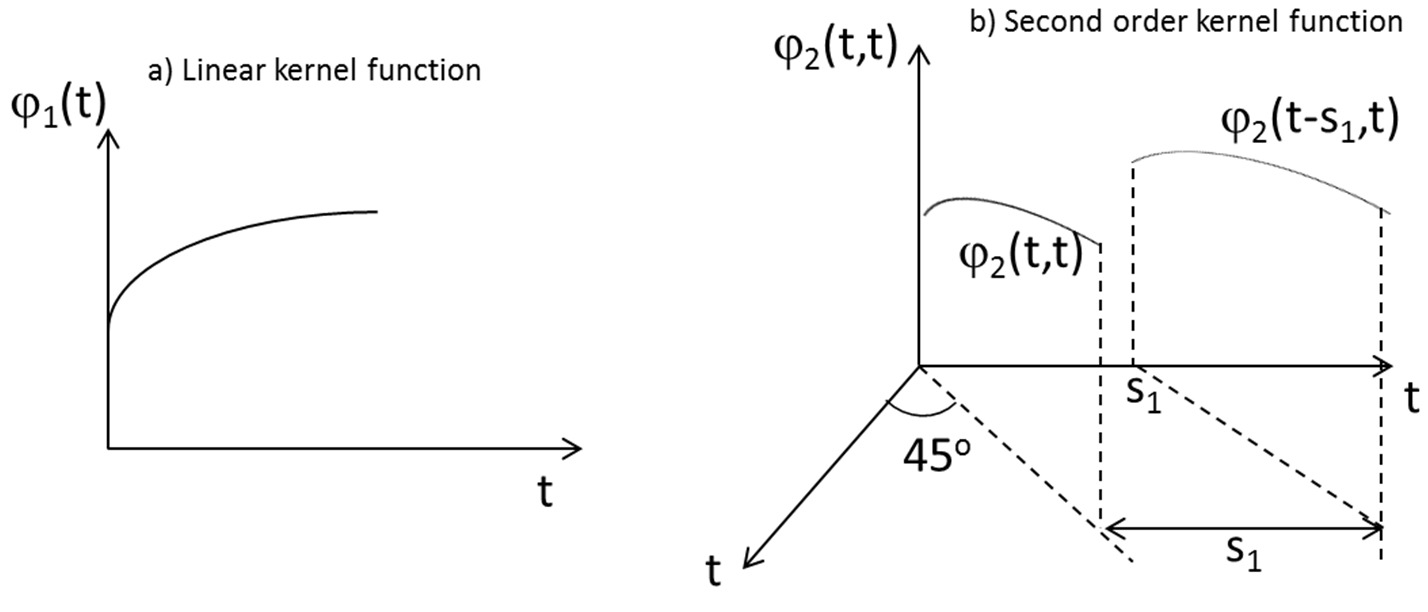
\includegraphics[width=5.0in]{./chap_3_minor_loop/figures/Time_dependent_kernel_functions.png}
\caption{The comparison between viscoelastic and elastic materials as host structure}
\label{fig:2.1.Time_dependent_kernel_functions}
\end{figure}
It is also assumed that the material response is unaltered by an arbitrary shift of the time scale, so that
 the following functions can be used for the two kernels in equation (\ref{EQN:double_integral_sample})

\begin{equation}
\begin{aligned}
 \psi_1(t-s)=& A_0+A_1 (1-e^{(-(t-s)/\tau_1)}) \\ 
 \psi_2(t-s_1,t-s_2) = & B_0+B_1 
\left(2-e^{-(t-s_1)/\lambda_1}-e^{-(t-s_2)/\lambda_2}\right)+ \\
& B_2\left(1-e^{(-(t-s_1)/\lambda_1)})(1-e^{(-(t-s_2)/\lambda_2)}\right)  
\end{aligned}
\label{EQN:double_integral_sample_second}
\end{equation}
where $A_0, A_1, B_0, B_1, \tau_1, \lambda_1, \lambda_2$ are the material parameters that need to be determined from experiments.
A set of experiments may be performed by applying the input variables at different times, say at $t=0$ and $t=s_1$.
The main disadvantage of the multiple integral forms is in difficulties characterizing the material parameters from experiments,
 even when only up to the second order kernel function is considered. 
The characterization of material parameters becomes even more complicated for the anisotropic and nonlinear time-dependent case,
 which is the case for piezoelectric ceramics. 
 In case of the third order term is included, the following third order kernel function can be considered.
\begin{equation}
\begin{aligned}
 \psi_3(t-s_1,t-s_2,t-s_3) = & C_0+C_1 
\left(3-e^{-(t-s_1)/\eta_1}-e^{-(t-s_2)/\eta_2}-e^{-(t-s_2)/\eta_3}\right)+ \\
& C_2\left(1-e^{(-(t-s_1)/\eta_1)}\right)  
     \left(1-e^{(-(t-s_2)/\eta_2)}\right)
     \left(1-e^{(-(t-s_3)/\eta_3)}\right)
\end{aligned}
\label{EQN:double_integral_sample_third_order}
\end{equation}
It is also necessary that  $\psi_3(t,t,t-s_1)=\psi_3(t-s_1,t,t)= \psi_3(t,t-s_1,t)$.
Detailed description of this method and its implementation for numerrical method is discussed in Sohrabi and Muliana \cite{Sohrabi2011}.

% \begin{figure}
% \centering
% \includegraphics[width=5.0in]
% {./chap_3_minor_loop/figures/fig_3_9_the_butterfly-like_shape_of_the_electro-mechanical_coupling_response.pdf}
% \caption{The butterfly-like shape of the electro-mechanical coupling response}
% \label{fig_3_9_the_butterfly_like_shape_of_the_electro_mechanical_coupling_response}
% \end{figure}

\section{Time Integration Method for Multiple Integral Form}
A numerical algorithm for determining time-dependent response from the multiple integral moduli is presented here. 
Let $R \left[ I(t-s),t \right] $ be the time-dependent response at current time $t \geq 0  $ due to an input history $I^s \equiv I(s) $

A general single integral representation for the response is: 

\begin{equation}
R^t \equiv R[I^s,t]=R[I^0,t]+\int_{0^+}^{t} \frac{\partial R}{\partial I}[I^s,t-s] \frac{d I^s}{d s} ds 
; (t \geq 0)
\label{2_15_eqn_Singel_integral}
\end{equation}
where
\begin{equation}
R[I^0,t]=R_0(I^0)+R_1 R(I^0) \left(1-exp \left[-\frac{t}{\tau_1} \right] \right)
\label{2_16_eqn_Singel_integral}
\end{equation}
and
\begin{equation}
\frac{\partial R}{\partial I}[I^s,t-s]=\frac{\partial R_0(I^s)}{\partial I}+\frac{\partial R_1(I^s)}{\partial I}
\left(1-exp \left[-\frac{t-s}{\tau_1} \right] \right)
\label{2_17_eqn_Singel_integral}
\end{equation}
Here a superscript is used to denote the time-dependent variables. 
A recursive method is used for solving the above integral form. 
Substituting equations (\ref{2_16_eqn_Singel_integral}) and (\ref{2_17_eqn_Singel_integral}) into equation (\ref{2_15_eqn_Singel_integral}) yields:
\begin{equation}
R^t=R_0(I^t)+R_1(I^t)-R_1(I^0) exp \left[-\frac{t}{\tau_1} \right]-q^t
\label{2_18_history_eqn_Singel_integral}
\end{equation}
where
\begin{equation}
q^t=\int_{0^+}^{t} \frac{\partial R_1 (I^s) }{\partial I} exp \left[-\frac{t-s}{\tau_1} \right] \frac{d I^s}{d s} ds
\label{2_19_history_eqn_Singel_integral}
\end{equation}
is the history variable, which can be approximated as: 
\begin{equation}
\begin{aligned}
&q^t \approx  exp \left[-\frac{-\Delta t}{\tau_1} \right] q^{t-\Delta t}+ 
\Big[\frac{\partial R_1 (I^t) } {\partial I} \frac{d I}{d s} \mid_t
+exp \left[ \frac{-\Delta t}{\tau_1} \right] \\  
&\frac{\partial R_1 (I^{t-\Delta t}) } {\partial I} \frac{d I}{d s} \mid_{t-\Delta t} \Big] \frac{\Delta t}{2}
\end{aligned}
\label{2_20_EQN:single_integral_history_variables}
\end{equation}
The superscript $t-\Delta t$ denotes the previous time history. 
At initial time, $q^t=q^0=0.0$ and $R^0=R_0(I^0)$. Equations (\ref{2_18_history_eqn_Singel_integral}) and (\ref{2_19_history_eqn_Singel_integral}) give the corresponding output due to an arbitrary input $I(s)$.
For the multi-axial constitutive relation, the approximate solution in equation (\ref{2_18_history_eqn_Singel_integral}) can be applied independently to each scalar component of constirutive equation.
The numerical algorithm for the multiple integral models (one-dimensional representation) with the kernels defined in equation (\ref{EQN:double_integral_sample_second}) can be approximated by applying the recursive method as discussed above. 
The linear kernel is approximated as:

\begin{equation}
\begin{aligned}
& \int_{s=0^{-}}^{t}  \psi_1(t-s) \frac{dI(s)}{d}ds \approx 
\left[ A_0+A_1 \right] I_t -A_1 I(0^+) exp \left[- \frac{t}{\tau_1} \right] -q^t_1\\
& q^t_1 \approx exp \left[- \frac{\Delta t}{\tau_1} \right] q^{t-\Delta t}_1 +A_1 \frac{\Delta t}{2} 
\left[ \frac{dI}{ds} \mid_t + exp \left[ - \frac{\Delta t}{\tau_1} \right]  \frac{dI}{ds} \mid_{t-\Delta t} \right]  \\
& t \geq 0 
\end{aligned}
\label{EQN_2.23:double_integral_expand}
\end{equation}

The second order kernel in equation (\ref{EQN:double_integral_sample}) is rewritten as:

\begin{equation}
\begin{aligned}
& \int_{s_1=0^{-}}^{t}\int_{s_2=0^{-}}^{t}\psi_2(t-s_1,t-s_2) \frac{dI(s_1)}{ds_1}ds_1 \frac{dI(s_2)}{ds_2}ds_2 =\\
& [B_0+B_1(2.-e^{-t/\lambda_1} -e^{-t/\lambda_1} ) +B_2 (1-e^{-t/\lambda_2}) (1-e^{-t/\lambda_2}) ]I(0^+)I(0^+)+ \\
& \int_{s_1=0^{-}}^{t}\int_{s_2=0^{-}}^{t}  \Big( B_0+B_1  \left(2-e^{-(t-s_1)/\lambda_1}-e^{-(t-s_2)/\lambda_2}\right)+ \\
& B_2\left(1-e^{(-(t-s_1)/\lambda_1)})(1-e^{(-(t-s_2)/\lambda_2)}\right) \Big)
 \frac{dI(s_1)}{ds_1}ds_1 \frac{dI(s_2)}{ds_2}ds_2 
\end{aligned}
\label{EQN_2.23:double_integral_expand_rewrited}
\end{equation}
It can be approximated by:
\begin{equation}
\begin{aligned}
& \int_{s_1=0^{-}}^{t}\int_{s_2=0^{-}}^{t}\psi_2(t-s_1,t-s_2) \frac{dI(s_1)}{ds_1}ds_1 \frac{dI(s_2)}{ds_2}ds_2 =\\
& [B_0+B_1(2.-e^{-t/\lambda_1} -e^{-t/\lambda_1} ) +B_2 (1-e^{-t/\lambda_2}) (1-e^{-t/\lambda_2}) ]I(0^+)I(0^+)+ \\
& (B_0+2B_1)( I(t)+I(0^+) )^2-B_1(I(t)+I(0^+))(f^t_1+g^t_1) +\\
& b_2( ( I(t)+I(0^+) )^2 -f^t_2( I(t)+I(0^+) )-g^t_2( I(t)+I(0^+) )+ f^t_2 g^t_2)
\end{aligned}
\label{2_24_EQN:double_integral_expand_approximated}
\end{equation}
where the history variables $f^t_1, f^t_2, g^t_1, g^t_2$ at $t>0.0$ are given as:
\begin{equation}
\begin{aligned}
& f^t_1 \approx  exp \left[-\frac{-\Delta t}{\lambda_1} \right] f^{t-\Delta t}_1+ \frac{\Delta t}{2} \left[  \frac{dI}{s_1} \mid_t+exp \left[ \frac{-\Delta t}{\lambda_1} \right]   \frac{dI}{s_1} \mid_{t-\Delta t} \right] \\
& g^t_1 \approx  exp \left[-\frac{-\Delta t}{\lambda_1} \right] g^{t-\Delta t}_1+ \frac{\Delta t}{2} \left[  \frac{dI}{s_2} \mid_t+exp \left[ \frac{-\Delta t}{\lambda_1} \right]   \frac{dI}{s_2} \mid_{t-\Delta t} \right] \\
& f^t_2 \approx  exp \left[-\frac{-\Delta t}{\lambda_2} \right] f^{t-\Delta t}_2+ \frac{\Delta t}{2} \left[  \frac{dI}{s_1} \mid_t+exp \left[ \frac{-\Delta t}{\lambda_2} \right]   \frac{dI}{s_1} \mid_{t-\Delta t} \right] \\
& g^t_2 \approx  exp \left[-\frac{-\Delta t}{\lambda_2} \right] g^{t-\Delta t}_2+ \frac{\Delta t}{2} \left[  \frac{dI}{s_2} \mid_t+exp \left[ \frac{-\Delta t}{\lambda_2} \right]   \frac{dI}{s_2} \mid_{t-\Delta t} \right] \\
\end{aligned} 
\label{2_25_EQN:double_integral_history_variables}
\end{equation}
It is noted that at initial time $f^0_1= f^0_2= g^0_1= g^0_2=0.0$ and $R(0)=A_0I(0^+)+B_0 I(0^+)I(0^+)$. 
Thus, the corresponding response due to an arbitrary input obtained from the multiple integral model is approximated as: 

\begin{equation}
\begin{aligned}
R(t) \approx 
&\left[A_0+ A_1 \right]I(t)-A_1 exp \left[- \frac{t}{\tau_1}\right] -q_1^t \\
&\left[B_0+B_1 (2-e^{-t/\lambda_1}-e^{-t/\lambda_1}) +B_2(1-e^{-t/\lambda_2})(1-e^{-t/\lambda_2}) \right]I(0^+)I(0^+)+ \\
&(B_0+2B_1)(I(t)-I(0^+))^2-B_1(I(t)-I(0^+))(f_1^t+g_1^t)+\\
&B_2\left[ (I(t)-I(0^+))^2 -f_2^t (I(t)-I(0^+)) -g_2^t (I(t)-I(0^+)) +f_2^t g_2^t\right]
\end{aligned} 
\label{2_26_EQN:double_integral_approximate_solution}
\end{equation}

For the multi-axial constitutive relation, the approximate solution in equation (\ref{2_26_EQN:double_integral_approximate_solution}) can be applied independently to each scalar component. 

\subsection{Multiple Integral Model}
This section presents a multiple integral model to simulate hysteretic response of a piezoelectric ceramics subject to a sinusoidal electric field. 
We consider up to the third order kernel function and we examine the effect of these kernel functions on the overall nonlinear hysteretic curve. 
The following material parameters are used for the simulation:
\begin{equation}
\begin{aligned}
&A_0=200 \cdot 10^{-12} m/V; A_2=100 \cdot 10^{-12} m/V \\
&\tau_1=2 sec \\
&B_0=B_1=B_2=20 \cdot 10^{-18} m^2/V^2 \\
&C_0=C_1=C_2=50 \cdot 10^{-24} m^3/V^3 \\
&\eta_1=2sec; \eta_2=5 sec  
\end{aligned}
\label{3_5_EQN:coefficients}
\end{equation}
When only the first and third kernel functions are considered, the nonlinear hysteretic response at steady state under positive and negative electric fields is identical as shown by an anti-symmetric hysteretic curve in figure \ref{figure_3_8_the_effect_of_the_higher_order_terms_on_the_hysteretic_response}a. 
The hysteretic response under the amplitude
of electric field of 0.25 MV/m shows nearly linear response. Including the second order
kernel function allows for different response under positive and negative electric fields as
seen in figure \ref{figure_3_8_the_effect_of_the_higher_order_terms_on_the_hysteretic_response}b. At low amplitude of applied electric field, nearly linear response is shown;
however this hysteretic response does not show an anti-symmetric shape with respect to the
strain and electric field axes. The contribution of each order of the kernel function depends
on the material parameters. For example the material parameters in equation (\ref{3_5_EQN:coefficients}) yield to more
pronounced contribution of the first order kernel function; while the contributions of the
second and third order kernel functions are comparable.

\begin{figure}
\centering
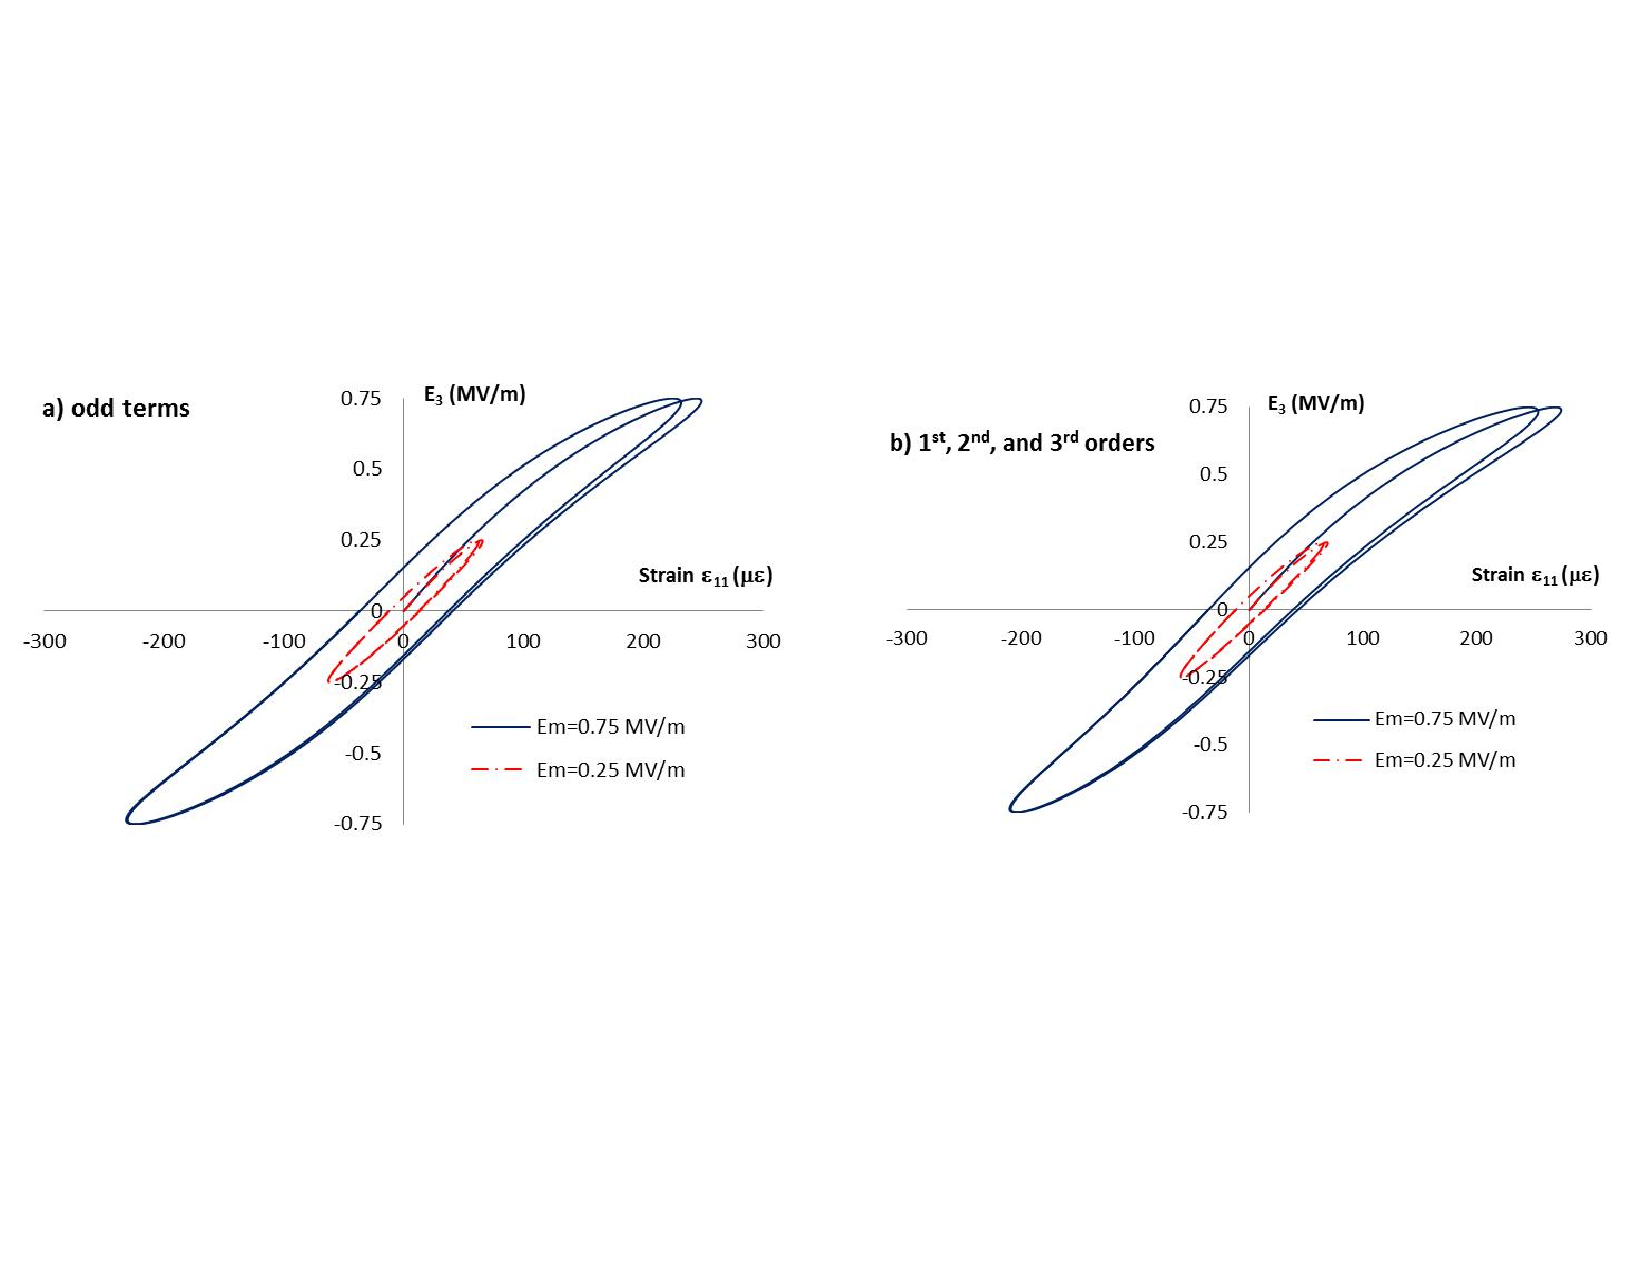
\includegraphics[width=6.0in]
{./chap_3_minor_loop/figures/figure_3_8_the_effect_of_the_higher_order_terms_on_the_hysteretic_response.pdf}
\caption{The effect of the higher order terms on the hysteretic response (f=0.1 Hz)}
\label{figure_3_8_the_effect_of_the_higher_order_terms_on_the_hysteretic_response}
\end{figure}

Intuitively, the corresponding strain response of a piezoelectric ceramics when an electric
field is applied in the poling direction (positive electric field) need not be the same as when
an electric field is applied opposite to the poling direction (negative electric field), especially
for nonlinear response due to high electric fields. Depoling could occur in the piezoelectric
ceramics when a negative electric field with a magnitude greater than the coercive electric
field is considered. Thus, to incorporate the possibility of the depoling process, the even
order kernel functions can be incorporated in the multiple time-integral model.  In order to
numerically simulate the depolarization in the piezoelectric ceramics we apply a sinusoidal
electric field input with amplitude of 1.5 MV/m. We consider the first and second order
kernel functions and use the following material parameters so that the contributions of the
first and second order kernel functions on the strain response are comparable:
\begin{equation}
\begin{aligned}
&A_0=200 \cdot 10^{-12} m/V; A_2=100 \cdot 10^{-12} m/V \\
&\tau_1=2 sec \\
&B_0=B_1=B_2=100 \cdot 10^{-18} m^2/V^2 \\
&\eta_1=2sec; \eta_2=5 sec  
\end{aligned}
\label{3_5_EQN:coefficients_}
\end{equation}

Figure \ref{fig_3_9_the_butterfly_like_shape_of_the_electro_mechanical_coupling_response} illustrates the corresponding strain response from the multiple integral model
having the first and second kernel functions. The response shows an un-symmetric
butterfly-like shape. The un-symmetric butterfly-like strain-electric field response is
expected for polarized ferroelectric materials undergoing high amplitude of sinusoidal
electric field input. The nonlinear response due to the positive electric field is caused by
different microstructural changes than the microstructural changes due to polarization
switching under a negative electric field. 

\begin{figure}
\centering
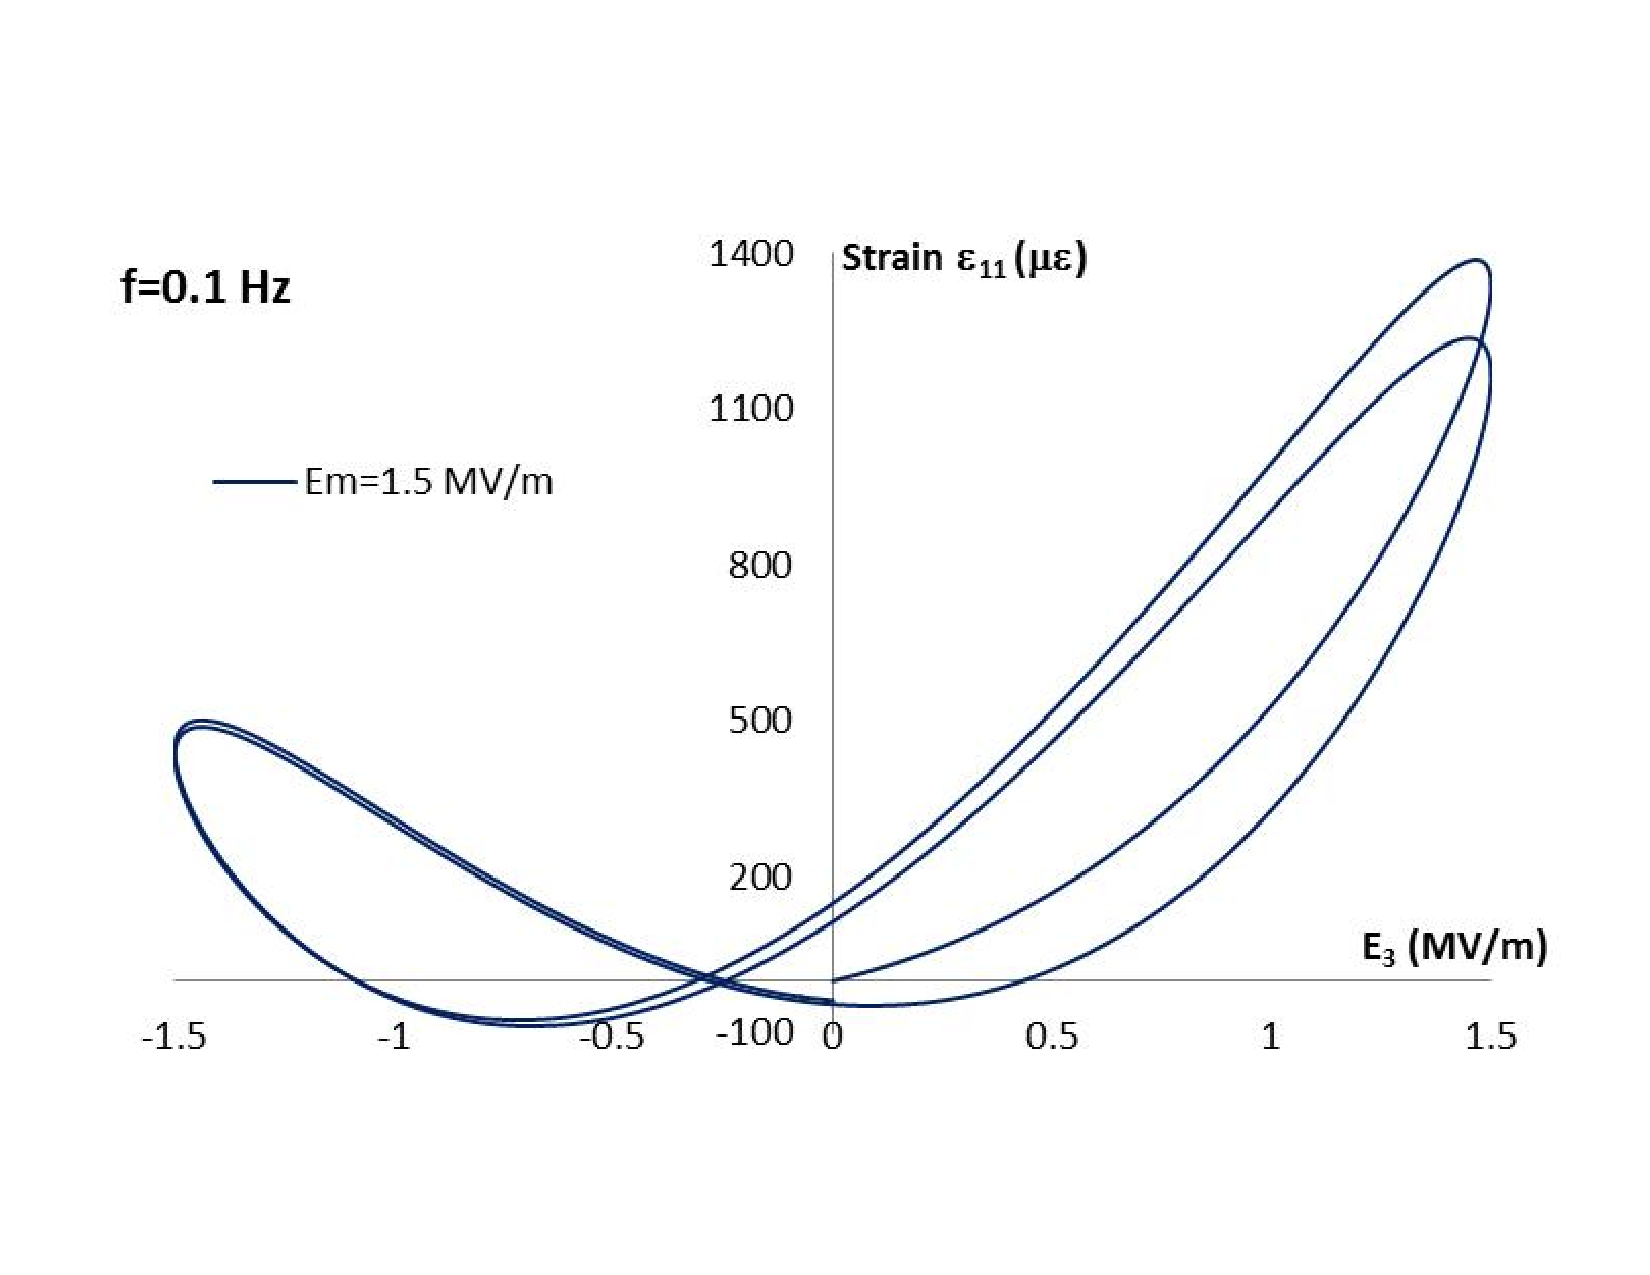
\includegraphics[width=5.0in]
{./chap_3_minor_loop/figures/fig_3_9_the_butterfly-like_shape_of_the_electro-mechanical_coupling_response.pdf}
\caption{The butterfly-like shape of the electro-mechanical coupling response}
\label{fig_3_9_the_butterfly_like_shape_of_the_electro_mechanical_coupling_response}
\end{figure}

\section{Quasi Linear Viscoelastic (QLV) Model \cite{sohrabi2015nonlinear}} 
In an analogy to a time-dependent deformation of visco-elastic materials \cite{Wineman2000}, 
a single integral representation for formulating time dependent electro-mechanical constitutive equations is also considered.
The time dependent electromechanical model is:  

\begin{equation}
\begin{aligned}
&\sigma_{ij}(t)=
\int_{0^-}^t 
\sum_{k,l=1}^3 \frac{\partial \sigma_{ij}}{\partial\varepsilon_{kl}}(t-s,\varepsilon_{kl}(s)) \dot{\varepsilon}_{kl}(s)ds-
\int_{0^-}^t
\sum_{k=1}^3 \frac{\partial \sigma_{ij}}{\partial E_{k}}(t-s,E_k(s)) \dot{E}_k(s)ds
\\
&D_k(t)=
\int_{0^-}^t 
\sum_{i,j=1}^3 \frac{\partial D_{k}}{\partial\varepsilon_{ij}}(t-s,\varepsilon_{ij}(s))\dot{\varepsilon}_{ij}(s)ds+
\int_{0^-}^t  
\sum_{i=1}^3 \frac{\partial D_{k}}{\partial E_{i}}(t-s,E_i(s)) \dot{E}_i(s) ds
\end{aligned}
\label{EQN:TimeIntegRepConstTensor}
\end{equation}
where the overdot indicates the time derivative, 
$t$ denotes the present time and $s$ is indicates the time history. 
It is assumed that all field variables at $t<0$ are zero, and loading starts at initial time $0$.
It is assumed that the time and field dependent parts can be separated by multiplicative decomposition\footnote{The separation of variables between the time and field dependent parts
was adopted from the quasi linear viscoelastic (QLV) model proposed by Fung
\cite{fung1981biomechanics}, which is used in many biological materials.}. 
Following the Quasi Linear Viscoelastic (QLV) model, the constitutive relation in equations (\ref{EQN:TimeIntegRepConstTensor}) can be further expressed in terms of the normalized time-dependent function \cite{tscharnuter2012nonlinear,fung1981biomechanics}, where it is written as:

\begin{equation}
\begin{aligned}
\sigma_{ij}(t)= 
&\int_{0^-}^t 
\sum_{k,l=1}^{3} K^C_{ijkl}(t-s)\frac{\partial \sigma_{ij}}{\partial\varepsilon_{kl}}(\varepsilon_{kl}(s))\dot{\varepsilon}_{kl}(s)ds +\\
&\int_{0^-}^t 
\sum_{k=1}^{3} K^e_{kij}(t-s) \frac{\partial \sigma_{ij}}{\partial E_{k}}(E_k(s))  \dot{E}_{k} (s)ds
\\
D_k(t)=
&\int_{0^-}^t 
\sum_{i,j=1}^{3} K_{kij}^e(t-s) \frac{\partial D_{k}}{\partial \varepsilon_{ij}}(\varepsilon_{ij}(s))\dot{\varepsilon}_{ij}(s)ds + \\
&\int_{0^-}^t 
\sum_{i=1}^{3} K_{ki}^{\kappa}(t-s) \frac{\partial D_{k}}{\partial E_{i}}(E_i(s))  \dot{E}_{i} (s)ds
\end{aligned}
\label{EQN:NormalizedConstitutiveRelation}
\end{equation} 
where $K^C_{ijkl}$, $K^e_{kij}$ and $K^{\kappa}_{ki}$ are the normalized time-dependent tensors corresponding to the elastic, electromechanical coupling, and permittivity tensor, respectively. 
The stresses $\sigma_{ij}$, and electric displacements  $D_k$, are evaluated at time $t$ and the input history is prescribed at $0^-<s<t$.
For the time-dependent constitutive relation, the kernel functions can be chosen to be general functions of time that are in accordance with the time-dependent behaviors,  e.g., relaxation or creep like behaviors, of the materials. 
In this study a series of discrete exponential functions, often called Prony series, is used for each time dependent kernel function.
The nonlinear time-dependent response discussed in this section can be used to model hysteresis electro-mechanical response of polarized piezoelectric ceramics under a cyclic electric field. 
The kernel functions are expressed as: 

\begin{equation}
\label{EQN:LrgKProny}
\begin{aligned}
&K_{ijkl}^C(t) =
\sum_{I=0}^{NP}{}^{I}K_{ijkl}^{C} exp(-{}^{I}\lambda_{ijkl}^{C}t) \\
&K_{ijk}^e(t) =
\sum_{I=0}^{NP} {}^{I}K_{ijk}^{e} exp(-{}^{I}\lambda_{ijk}^{e}t) \\
&K_{ki}^\kappa(t) =
\sum_{I=0}^{NP}  {}^{I}K_{ki}^{\kappa} exp(-{}^{I}\lambda_{ki}^{\kappa}t) \\
\end{aligned}
\end{equation}                   
where $ {}^{I}K_{ijkl}^{C} $, $ {}^{I}K_{ijk}^{e} $, $ {}^{I}K_{ki}^{\kappa} $ , $ {}^{I}\lambda_{ijkl} $, $ {}^{I}\lambda_{ijk}^{e} $, and $ {}^{I}\lambda_{ki}^{\kappa} $ are the material parameter related to $ I^{th} $ component of Prony series of $ K_{ijkl}^C(t) $, $ K_{ijk}^e(t) $, and  $ K_{ki}^\kappa(t) $.
Equation (\ref{EQN:LrgKProny}) defines the time dependent functions, corresponding to the electro-mechanical properties.
The chosen time-dependent functions for material properties, either creep or relaxation function, are determined based on the experimental data. 
It is also possible that some terms in the properties experience relaxation and other terms experience creep responses. 
Zhou and Kamlah \cite{zhoudetermination2005} and Anderson \cite{anderson1989piezoceramic} performed experiment on PZT ceramics.
They have shown that the electric displacement in the tested piezoelectric ceramics increases with time when a constant electric field is prescribed. 
In such cases, the time-dependent electric permittivity constants should follow creep functions. 
It has also been shown that piezoelectric ceramics experience creep deformation due to constant stress, or they undergo stress relaxation when constant strain is prescribed.

When mathematical models with rather simple forms are considered for the input history and time-dependent material properties,
it is possible to obtain exact analytical solutions for the nonlinear time dependent constitutive equation.
Laplace transform method \cite{Wineman2000} is often used to determine the corresponding time-dependent field variables for the linear response of materials. 
Piezoelectric ceramics exhibit nonlinear electro-mechanical response under a relatively large magnitude of electric field. 
In dealing with nonlinear responses, numerical methods are considered for obtaining solutions to the governing equations.
Recursive integration technique has been shown to be very effective in solving the nonlinear integral problem. 
In this study, a numerical method based on the recursive approach is adopted for solving the nonlinear time-dependent electro-mechanical coupling response.
This numerical technique will be integrated into FE analyses that is explained in following sections.

Using the time dependent constitutive equations that were presented in equation (\ref{EQN:NormalizedConstitutiveRelation}) and the time kernel function that is expressed as series of exponential functions as equation (\ref{EQN:LrgKProny}) with $ {}^{I}\lambda_{ijkl}=0$, $ {}^{I}\lambda_{ijk}^{e}=0$, and $ {}^{I}\lambda_{ki}^{\kappa}=0$, 
the expanded constitutive equations are written as:
\begin{equation}
\begin{aligned} 
\sigma_{ij}(t)=
&\sum_{k,l=1}^{3} {}^{0}K_{ijkl}^{C} 
\frac{\partial \sigma_{ij}}{\partial \varepsilon_{kl}}(\varepsilon_{kl}(t)) \varepsilon_{kl}(t)+
\sum_{k=1}^{3}
{}^{0}K_{ijk}^{e}\frac{\partial \sigma_{ij}}{\partial E_{k}}(E_{k} (t)) E_{k} (t) +\\
&\int_{0^-}^t 
\sum_{k,l=1}^{3} 
\sum_{I=1}^{NP}{}^{I}K_{ijkl}^{C} exp(-{}^{I}\lambda_{ijkl}^{C}[t-s]) 
\frac{\partial \sigma_{ij}}{\partial
\varepsilon_{kl}}(\varepsilon_{kl}(s)) \dot{\varepsilon}_{kl}(s)ds +\\
&\int_{0}^t 
\sum_{k=1}^{3}
\sum_{I=1}^{NP}
{}^{I}K_{ijk}^{e}
exp(-{}^{I}\lambda_{ijk}^{e}[t-s]) \frac{\partial \sigma_{ij}}{\partial E_{k}} (E_{k} (s)) \dot{E}_{k} (s)ds
\end{aligned}
\label{EQN:RecursiveProny_stress}
\end{equation}

\begin{equation}
\begin{aligned} 
D_k(t)=
&\sum_{i,j=1}^{3}
{}^{0}K_{ijk}^{e}\frac{\partial
D_{k}}{\partial \varepsilon_{ij}} (\varepsilon_{ij}(t)) \varepsilon_{ij}(t)+
\sum_{i=1}^{3}
{}^{0}K_{ki}^{\kappa}\frac{\partial D_{k}}{\partial E_{i}}(E_{i} (t)) E_{i} (t)+\\
&\int_{0^-}^t 
\sum_{i,j=1}^{3}  
\sum_{I=1}^{NP}
{}^{I}K_{ijk}^{e} exp(-{}^{I}\lambda_{ijk}^{e}(t-s))
\frac{\partial D_{k}}{\partial \varepsilon_{ij}}(\varepsilon_{ij}(s))\dot{\varepsilon}_{ij}(s)ds+\\
&\int_{0^-}^t 
\sum_{i=1}^{3} 
\sum_{I=0}^{NP}
{}^{I}K_{ki}^{\kappa}exp(-{}^{I}\lambda_{ki}^{\kappa}[t-s]) \frac{\partial D_{k}}{\partial E_{i}} (E_{i} (s)) \dot{E}_{i} (s)ds
\end{aligned}
\label{EQN:RecursiveProny_elect_disp}
\end{equation}

Equations (\ref{EQN:RecursiveProny_stress}, \ref{EQN:RecursiveProny_stress}) are rewritten with the definition of history variables as follows:

\begin{equation}
\begin{aligned}
\sigma_{ij}(t)=
&\sum_{k,l=1}^{3}  
{}^{0}K_{ijkl}^{C} 
\frac{\partial \sigma_{ij}}{\partial \varepsilon_{kl}}(\varepsilon_{kl}(t))\varepsilon_{kl}(t)+
\sum_{k,l=1}^{3} 
\sum_{I=1}^{NP}
{}^{I}q_{ijkl}^{\sigma_C}(t) + \\
&
\sum_{k=1}^{3}
{}^{0}K_{ijk}^{e}\frac{\partial \sigma_{ij}}{\partial E_{k}}(E_{k} (t)) E_{k} (t)+ 
\sum_{k=1}^{3} 
\sum_{I=1}^{NP}{}^{I}q_{ijk}^{\sigma_e}(t)\\
D_k(t)=
&\sum_{i,j=1}^{3}
{}^{0}K_{ijk}^{e}\frac{\partial D_{k}}{\partial \varepsilon_{ij}}(\varepsilon_{ij}(t)) \varepsilon_{ij}(t)+
\sum_{i,j=1}^{3}
\sum_{I=1}^{NP}{}^{I}q_{kij}^{D_e}(t) +\\
&
\sum_{i=1}^{3}
{}^{0} K_{ki}^{\kappa}\frac{\partial D_{k}}{\partial E_{i}}(E_{i} (t)) E_{i} (t)+ 
\sum_{i=1}^{3}
\sum_{I=1}^{NP}
{}^{I}q_{ki}^{D_{\kappa}}(t)
\end{aligned}
\label{EQN:History_Introduction}
\end{equation}
where the variables ${}^{I}q_{ijkl}^{\sigma_C}(t) $, ${}^{I}q_{ijk}^{\sigma_e}(t)$, ${}^{I}q_{kij}^{D_e}(t)$ and ${}^{I}q_{ki}^{D_{\kappa}}(t)$ are defined to incorporate the history in the time integral constitutive equations. 
The time integral functions are split into two parts, the first part carries the integral from the beginning to the time ($t-\Delta t$) and the second part incorporates the integral within an incremental time $\Delta t$. 
The recursive method is used for all the integrations. 
Consider a simple integral with an exponential function such as $q(t)=\int_0^t exp(-\lambda [t-s])f(s)ds$.
This integral can be approximated as $q(t)\approx exp(-\lambda\Delta t) q(t-\Delta t) +\frac{\Delta t}{2} [f(t)+exp(-\lambda \Delta t ) f(t-\Delta t)]$.
This recursive scheme is used for solving the time dependent constitutive equations. 
Using the recursive integral, the history variables are given as:   

\begin{equation}
\begin{aligned}
{}^{I}q_{ijkl}^{\sigma_C}(t)= 
&exp(-{}^{I}\lambda_{ijkl}^{C}[\Delta t]){}^{I}q_{ijkl}^{\sigma_C}(t-\Delta t)+ \\
&\int_{t-\Delta t}^{t}  
{}^{I}K_{ijkl}^{C}
exp(-{}^{I}\lambda_{ijkl}^{C}[t-s])\frac{\partial \sigma_{ij}}{\partial \varepsilon_{kl}} (\varepsilon_{kl}(s)) \dot{\varepsilon}_{kl}(s)ds \\
{}^{I}q_{ijk}^{\sigma_e}(t)=
&exp(-{}^{I}\lambda_{ijk}^{e}[\Delta t]) {}^{I}q_{ijk}^{\sigma_e}(t-\Delta t)+ \\
&\int_{t-\Delta t}^{t}  
{}^{I}K_{ijk}^{e} exp(-{}^{I}\lambda_{ijk}^{e}[t-s]) \frac{\partial \sigma_{ij}}{\partial E_{k}} (E_{k} (s)) \dot{E}_{k} (s)ds \\
{}^{I}q_{ijk}^{D_e}(t)=
&exp(-{}^{I}\lambda_{ijk}^{e}[\Delta t]){}^{I}q_{ijk}^{D_e}(t-\Delta t)+\\
&\int_{t-\Delta t}^t 
{}^{I}K_{ijk}^{e} exp(-{}^{I}\lambda_{ijk}^{e}[t-s]) \frac{\partial D_{k}}{\partial \varepsilon_{ij}}(\varepsilon_{ij}(s)) \dot{\varepsilon}_{ij}(s)ds\\
{}^{I}q_{ki}^{D_{\kappa}}(t)=
&exp(-{}^{I}\lambda_{ki}^{\kappa}[\Delta t]){}^{I}q_{ki}^{D_{\kappa}}(t-\Delta t)+\\
&\int_{t-\Delta t^-}^t  
{}^{I}K_{ki}^{\kappa}
exp(-{}^{I}\lambda_{ki}^{\kappa}[t-s]) \frac{\partial D_{k}}{\partial E_{i}} (E_{i} (s)) \dot{E}_{i} (s)ds
\end{aligned}
\label{EQN:History_Discritizing}
\end{equation}
The above equations only need to be integrated within a time increment $\Delta t$. 
An approximate form of the time derivatives of field variables is taken as: $\dot{\varepsilon}_{kl} \approx \frac{\Delta \varepsilon_{kl}}{\Delta t}$ and $\dot{E}_{k}\approx \frac{\Delta E_k}{\Delta t}$. 
Upon solving the integrals in equation (\ref{EQN:History_Discritizing}) the history variables are:
\begin{equation}
\begin{aligned}
{}^{I}q_{ijkl}^{\sigma_C}(t)=&
exp(-{}^{I}\lambda_{ijkl}^{C}[\Delta t]){}^{I}q_{ijkl}^{\sigma_C}(t-\Delta t)+ \\
& \frac{{}^{I}K_{ijkl}^{C}}{2} \Big(exp(-{}^{I}\lambda_{ijkl}^{C}[\Delta t])\frac{\partial \sigma_{ij}}{\partial \varepsilon_{kl}}(\varepsilon_{kl}(t-\Delta t)) \Delta\varepsilon_{kl}(t-\Delta t) + \\
& \frac{\partial \sigma_{ij}}{\partial \varepsilon_{kl}}(\varepsilon_{kl}(t)) \Delta \varepsilon_{kl}(t) \Big) \\
{}^{I}q_{ijk}^{\sigma_e}(t)=&
 exp(-{}^{I}\lambda_{ijk}^{e}[\Delta t]) {}^{I}q_{ijk}^{\sigma_e}(t-\Delta t)+ \\
& \frac{{}^{I}K_{ijk}^{e}}{2} \Big( exp(-{}^{I}\lambda_{ijk}^{e}[\Delta t]) \frac{\partial \sigma_{ij}}{\partial E_{k}}(E_{k} (t-\Delta t )) \Delta E_{k} (t-\Delta t ) + \\
& \frac{\partial \sigma_{ij}}{\partial E_{k}} (E_{k} (t)) \Delta E_{k} (t) \Big)\\
\end{aligned}
\label{EQN:History_Discritizing_Breaking_Integral_1_2}
\end{equation}
\begin{equation}
\begin{aligned}
{}^{I}q_{ijk}^{D_e}(t)=&
exp(-{}^{I}\lambda_{ijk}^{e}[\Delta t]){}^{I}q_{k}^{D_e}(t-\Delta t)+\\
& \frac{{}^{I}K_{ijk}^{e}}{2} \Big(exp(-{}^{I}\lambda_{ijk}^{e}[\Delta t]) \frac{\partial D_{k}}{\partial \varepsilon_{ij}}( \varepsilon_{ij}(t-\Delta t)) \Delta \varepsilon_{ij}(t-\Delta t) + \\
& \frac{\partial D_{k}}{\partial \varepsilon_{ij}}(\varepsilon_{ij}(t)) \Delta \varepsilon_{ij}(t)\Big) \\
{}^{I}q_{ki}^{D_{\kappa}}(t)=&
exp(-{}^{I}\lambda_{ki}^{\kappa}[\Delta t]){}^{I}q_{k}^{D_{\kappa}}(t-\Delta t)+\\
& \frac{{}^{I} K_{ki}^{\kappa}}{2} \Big( exp(-{}^{I}\lambda_{ki}^{\kappa}[\Delta t]) \frac{\partial D_{k}}{\partial E_{i}}( E_{i} (t-\Delta t)) \Delta E_{i} (t-\Delta t) + \\ 
& \frac{\partial D_{k}}{\partial E_{i}}( E_{i} (t)) \Delta E_{i} (t)\Big)
\end{aligned}
\label{EQN:History_Discritizing_Breaking_Integral_3_4}
\end{equation}

Equations (\ref{EQN:History_Introduction}) and (\ref{EQN:History_Discritizing_Breaking_Integral_1_2}, \ref{EQN:History_Discritizing_Breaking_Integral_3_4}) give an approximate solutions of nonlinear-time-dependent constitutive equations. 
In the above equations the strain and electric field at each time increment are the independent variables that will be determined from structural analyses.

\section{Finite Element Implementation of QLV Model}
\label{Chapter:Finite_element}
This section briefly presents a FE formulation for analyzing the nonlinear time-dependent electro-mechanical responses of piezoelectric devices. 
At structural scale, displacement and electric potential are taken as independent field variables, which are sampled at nodes in finite elements. 
At the material scale (Gaussian integration points), strains and electric fields are the independent field variables, which are determined from equations (\ref{EQN:Linear_Displacement}) and (\ref{EQN:Linear_Electric_Field}), respectively.
At material points the constitutive model discussed in the previous section is used to determine the corresponding stress and electric displacements. 
General FE formulations for linear and time-independent electro-mechanical response of piezoelectric materials can be found in \cite{Benjeddou2000}.
This study focuses on nonlinear time dependent electro-mechanical responses of piezoelectric materials and structures. 

Consider a 3D continuum element placed in a Cartesian coordinates $x_1, x_2, x_3$. 
Let $[u]^T=[u_1,u_2,u_3,\phi]^T$ be the element field variables (displacements and electric potential). 
The nodal displacement and electric potential on the element are:
\begin{equation}
[d]^T=[u_1^1,u_2^1,u_3^1,\phi^1 \dots u_1^{nne},u_2^{nne},u_3^{nne},\phi^{nne}]
\label{EQN:dof_vector_structure}
\end{equation}
where $nne$ is the number of nodes in an element.
The field variables in the element $u_i$ are at the nodes $d_i$ are related by the shape function matrix $\varphi_{ip}$ as follows:

\begin{equation}
u_i=
\sum _{p=1}^{ndfe} \varphi_{ip} d_p,(i=1\dots nne)
\label{EQN:DispShapeDof}
\end{equation}
where $ndfe$ is number of degrees of freedom in each node.
The same shape functions are used for the displacement and electric potential field variables. 
To solve the nonlinear equation, the analyses start with trial linearized relations, followed by an iteration at each time increment 
in order to minimize error from linearizing the nonlinear equations.
At each time increment and at each material point, the constitutive relations in equation (\ref{EQN:NormalizedConstitutiveRelation}) are implemented. 
The incremental solution method given in equations (\ref{EQN:History_Introduction})-(\ref{EQN:History_Discritizing_Breaking_Integral_1_2}, \ref{EQN:History_Discritizing_Breaking_Integral_3_4}) is used.
The finite element analysis based on variational principle is considered for solving the equilibrium equations and determining the field variables.
The virtual work for the  electro-mechanically coupled system is \cite{Benjeddou2000,tiersten1993electroelastic}:
\begin{equation} 
\begin{aligned}
\delta \pi= 
& \int_V 
\sum_{i,j=1}^3 \sigma_{ij}\delta \varepsilon_{ij} dV -
\int_V 
\sum_{i=1}^3 D_{i}\delta E_{i} dV- \\
&\int_{\partial V}
\sum_{i=1}^3 T_{i}\delta u_{i} d{\partial V}+
\int_{\partial V} 
Q\delta \phi d{\partial V}
\label{EQN:Variation_of_Energy}
\end{aligned}
\end{equation}
where $T_{i}$ and $u_{i}$ denote the components of the surface traction and mechanical displacement vector, respectively.
Moreover, $Q$ and $\phi$ are the surface charge and scalar potential, respectively.
Definition of strain in equation (\ref{EQN:Linear_Displacement}) and electric field in equation (\ref{EQN:Linear_Electric_Field}), are used in the virtual work in equation (\ref{EQN:Variation_of_Energy}). 
The virtual work is now presented as a function of degrees of freedom and their variation, which are $[u_1,u_2,u_3,\phi]^T$ and $[\delta u_1,\delta u_2,\delta u_3,\delta \phi]^T$. 
In forming the equilibrium equations, the derivative of the virtual work with respect to the degrees of freedom is taken and set equal to zero:
\begin{equation}
R_k=\frac{\partial \delta \pi}{\partial \delta d_k}=0 ,(k=1\dots ndf)
\label{EQN:ResidualRepresentation}
\end{equation}
where $R_k$ is residual. Equation (\ref{EQN:ResidualRepresentation}) represents a system of nonlinear equations with respect to degrees of freedom whose solution is obtained at each time increment. 
By substituting the virtual work in equation (\ref{EQN:Variation_of_Energy}) into the residual in equation (\ref{EQN:ResidualRepresentation}) we have:

\begin{equation}
\begin{aligned}
R_k=
& \int_V 
\sum_{i,j=1}^3 \sigma_{ij} \frac{\partial \varepsilon_{ij}}{\partial \delta d_k}dV-
\int_V 
\sum_{i=1}^3 D_{i} \frac{\partial \delta E_{i}}{\partial \delta d_k}  dV- \\
& \int_{\partial V} \sum_{i=1}^3 T_{i} \frac{\partial \delta u_{i}}{\partial \delta d_k}  d{\partial V}+
\int_{\partial V} 
Q \frac{\partial \delta \phi}{\partial \delta d_k}  d{\partial V} 
\end{aligned}
\label{EQN:Residual_Variation_of}
\end{equation}

The derivative of strain and electric field that appears in the above equation contain the derivatives of the shape functions. 
Using the approximation functions in equation (\ref{EQN:DispShapeDof}) for the field variables and definition of strain and electric field in equations (\ref{EQN:Linear_Displacement}) and (\ref{EQN:Linear_Electric_Field}) we have:

\begin{equation}
\begin{aligned}
&\frac{\partial \delta \varepsilon_{ij}}{\partial \delta d_k}=\frac{\varphi_{ik,j}+\varphi_{jk,i}}{2} \\
&\frac{\partial \delta E_{i}}{\partial \delta d_k}= \varphi_{4k,i}\\
\end{aligned}
\label{EQN:Shape_Fucntion_Derivitive}
\end{equation}

This system of equations is solved iteratively.  
In this study, the Newton-Raphson iterative method is used to determine the field variables by satisfying $\Vert R_k \Vert \leq \epsilon_0$ for the entire structure ($\epsilon_0$ is the convergence tolerance).
The corrected field variables from the Newton-Raphson iterative methods for solving the nonlinear equation (\ref{EQN:ResidualRepresentation}) are obtained from:
\begin{equation}
R_k^{r}=- \frac{\partial R_k^{r-1}}{\partial d_k^{r-1}} (d_k^{r}-d_k^{r-1})
\label{EQN:Newton_Raphson_Iteration}
\end{equation}
where $r$ is the iteration counter and $d_k^{r}$ is degrees of freedom vector for the entire structure. 
From equation (\ref{EQN:Newton_Raphson_Iteration}), the Newton-Raphson method requires finding the tangent matrix $\frac{\partial R_k^{r}}{\partial d_k^{r}}$ in each iteration and at each time increment. 
The consistent tangent matrix is defined as:

\begin{equation}
\begin{aligned}
\mathcal{K}_{kl}=
& \frac{\partial R_k}{\partial d_l}= 
\frac{\partial}{\partial d_l} \frac{\partial \delta \pi}{\partial \delta d_k}= \\
& \sum_{i,j=1}^3 \frac{\partial R_k}{\partial \varepsilon_{ij}}\frac{\partial \varepsilon_{ij}}{\partial d_l}+  
 \sum_{i=1}^3 \frac{\partial R_k}{\partial E_{i}}\frac{\partial E_{i}}{\partial d_l}\\ 
& (l,k=1\dots ndf)
\end{aligned}
\label{EQN:TangentRepresentation}
\end{equation}  
where $ndf$ is the number of degrees of freedom.
The derivative terms in the above equation are defined:

\begin{equation}
\begin{aligned}
&\frac{\partial R_k}{\partial \varepsilon_{ij}}=
\int_V  
\sum_{m,n=1}^3 \frac{\partial \sigma_{mn}}{\partial \varepsilon_{ij}} \frac{\partial \delta \varepsilon_{mn}}{\partial \delta d_k}  dV-
\int_V 
\sum_{p=1}^3 \frac{\partial D_{p}}{\partial \varepsilon_{ij}}  \frac{\delta E_{p}}{\partial \delta d_k} dV  \\
&\frac{\partial R_k}{\partial E_{i}}=
\int_V  
\sum_{m,n=1}^3 \frac{\partial \sigma_{mn}}{\partial E_{i}} \frac{\partial \delta \varepsilon_{mn}}{\partial \delta d_k}  dV-
\int_V 
\sum_{p=1}^3 \frac{\partial D_{p}}{\partial E_{i}}  \frac{\delta E_{p}}{\partial \delta d_k} dV  \\
& (k=1\dots ndf)
\end{aligned}
\label{EQN:StressExplcitTangent}
\end{equation}
For the nonlinear and time dependent electro-mechanical  response, the material
derivatives in equations (\ref{EQN:Non_LinearLinear_Constants}) 
and time representation of stress and electric field are used in the above equation.

\section{Numerical Implementation}
\subsection{Analyses of Nonlinear Electro-Mechanical Response}
The experimental data of piezoelectric ceramics reported in \cite{Crawley1990} are first used to validate the constitutive model.
Calibrating the material properties is a rather non trivial task.
The first guess starts with the linear and time independent response.
In order to calibrate the material parameter in proposed constitutive model, we use the coupling coefficient $d_{ijk}$ in the constitutive equation, $\varepsilon_{11}=-d_{311}E_3$. 
The coupling coefficients $d_{ijk}$ are related to the stress coupling coefficients $e_{ijk}$ \cite{Leo2007}. 
The experiment was conducted on G-1195 PZT where the sample was excited with electric field at frequency 0.1Hz and three different amplitudes: $250 V/mm, 500 V/mm$ and $750 V/mm$.


In case a linear and time independent model is considered for the piezoelectric response of this material there will not be any hysteresis response, as shown in figure \ref{fig:Crawley_xp_TimeinDepenLin}. 
The material constant $d_{311}$, is taken to be $340 pm/V$ in order to match the strain at $500 V/mm$. 
In order to compare the piezoelectric constant $d_{311}$ of G-1195 PZT with other testing data under small electric field (linear range), the $d_{311}$ value of $180 pm/V$ \cite{low1995modeling} is alo plotted in figure \ref{fig:Crawley_xp_TimeinDepenLin}.

\begin{figure} 
\centering 
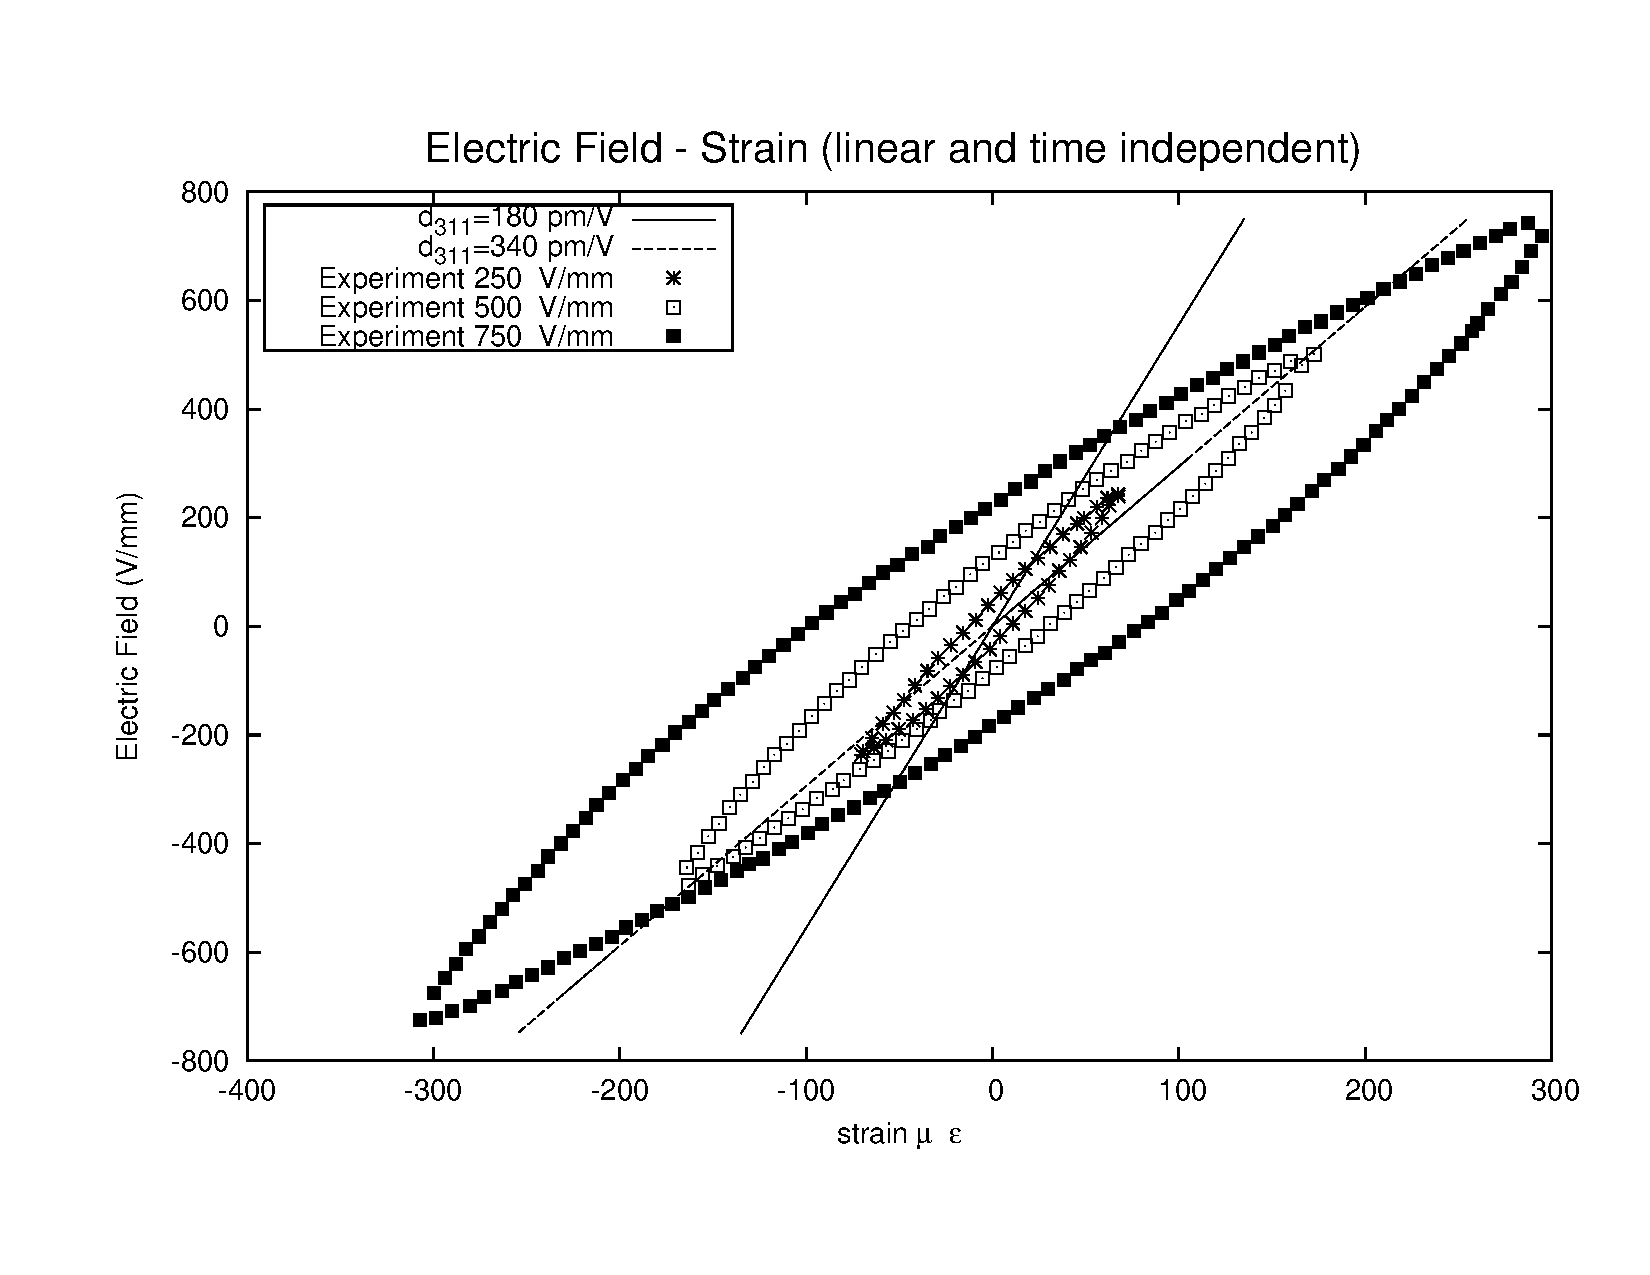
\includegraphics[width=5.0in]{./chap_3_minor_loop/figures/crawley_linear_time_independent.pdf}
\caption{Linear time independent model compared with experimental strain ($\varepsilon_{11}$) response under electric field ($E_3$) with frequency 0.1 Hz in \cite{Crawley1990}}
\label{fig:Crawley_xp_TimeinDepenLin}
\end{figure}
 
\begin{figure} 
\centering
\includegraphics[width=5.0in]{./chap_3_minor_loop/figures/crawley_linear_time_dependent-eps-converted-to.pdf}
\caption{Linear and history dependent model compared with experimental strain ($\varepsilon_{11}$) response under electric field ($E_3$) with frequency 0.1 Hz in \cite{Crawley1990}}
\label{fig:Crawley_xp_His_dependent_Lin}
\end{figure}

We use the model in equation (\ref{EQN:RecursiveProny_stress}, \ref{EQN:RecursiveProny_stress}) \cite{tscharnuter2012nonlinear} to include the effect of loading history. 
The time kernel function with $K(t)=1.0-0.6 exp(-t/1.2)$ in considered within the integral representation for the strain $\varepsilon_{11}(t)=\int_0^t
K(t-s)\frac{\partial \varepsilon_{11}}{\partial E_3}\frac{\partial
E_3(s)}{\partial s} ds$ with $\frac{\partial \varepsilon_{11}}{\partial
E_3}=-d_{311}$ taken to be $340 pm/V$ and the model shows a better result compared to the experiment under amplitude of $250V/mm$ as seen in figure \ref{fig:Crawley_xp_His_dependent_Lin}. 
It is clear from these results that the response of this material, even for small strain, is nonlinear, therefore taking $\frac{\partial\varepsilon_{11}}{\partial E_3}$ as a constant leads to some error when large electric field is considered.
As it is suggested in the literature \cite{anderson1989piezoceramic,Crawley1990} the piezoelectric coefficient should be defined as a function of applied electric field (they showed that $d_{311}$ changes linearly with strain and also electric field).
In this analysis we include the quadratic function of electric field. 
Following the same procedure as \cite{tscharnuter2012nonlinear} we define a nonlinear response function $\varepsilon_{11}(E_3)=-d_{311}^0 E_3-d_{311}^1 |E_3| E_3$.
Here we take $d_{311}^0=340pm/V$ and\footnote{$f$ here stands for femto i.e. $10^{-15}$ } $d_{311}^1=0.71 fm^2/V^2 $ the result from this calibration is shown in figure \ref{fig:TimeDepenNonLinCrawley}. It is seen that the hysteresis strain and electric field curves under several amplitude of electric field at frequency 0.1 Hz determined from the model are in good correlation with experimental data.
As discussed previously, it is possible to consider only odd terms in the higher order terms of the nonlinear constitutive relation.
Another nonlinear model incorporating first and third order terms is considered, e.g. $\varepsilon_{11}(E_3)=-d_{311}^0 E_3-d_{311}^2 E_3^3$ with $d_{311}^0=340pm/V$ and $d_{311}^2=0.55 z m/V$ \footnote{$z$ here stands for Zepto i.e. $10^{-21}$ } using the time dependent parameter discussed above ($K(t)=1.0-0.6 exp(-t/1.2)$), 
the nonlinear and time dependent model can capture the hystersis response under different amplitude of electric fields, as shown in figure \ref{fig:TimeDepenNonLinCrawleyThirdordermodel}. 
\begin{figure}
\centering
\includegraphics[width=5.0in]
{./chap_3_minor_loop/figures/crawley_non_linear_time_dependent-eps-converted-to.pdf}
\caption{Nonlinear time dependent strain ($\varepsilon_{11}$) response under electric field ($E_3$) with frequency 0.1 Hz compared with experiment \cite{Crawley1990}.}
\label{fig:TimeDepenNonLinCrawley}
\end{figure}

\begin{figure}
\centering
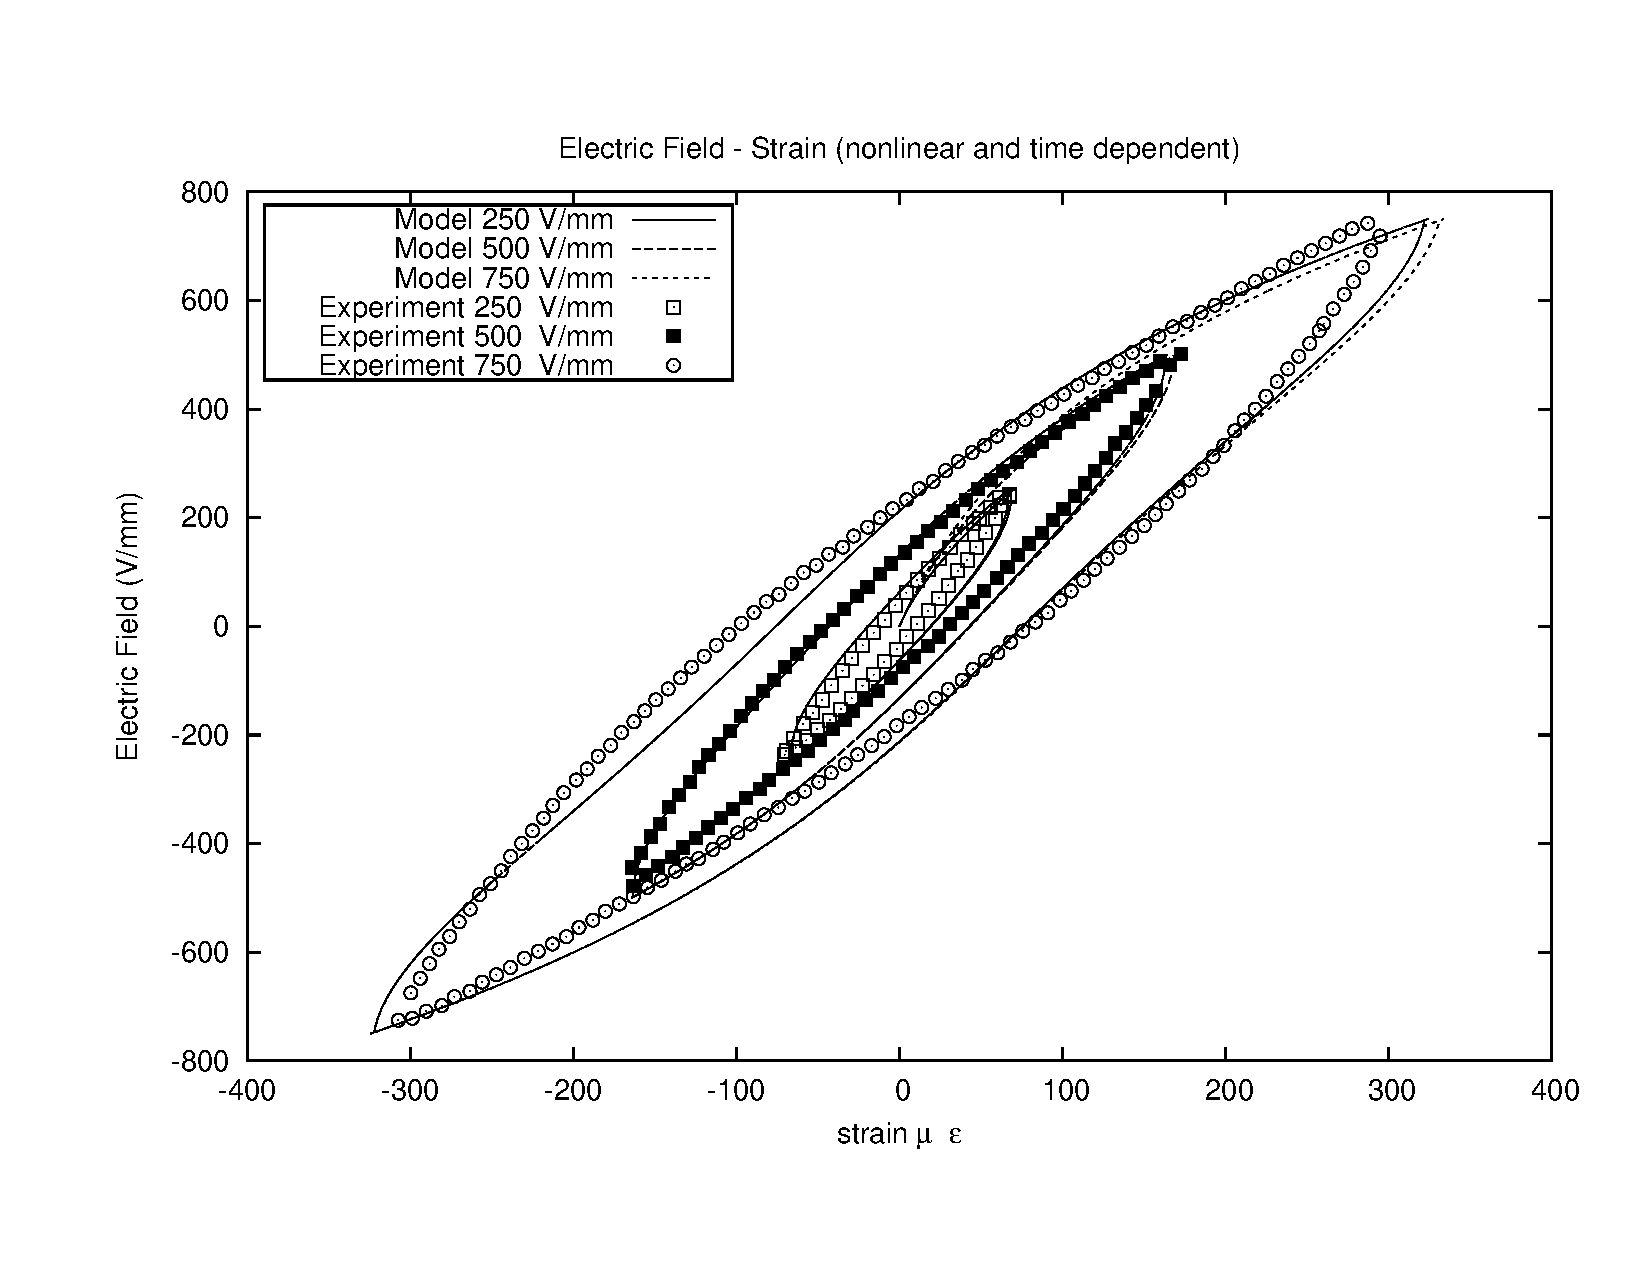
\includegraphics[width=5.0in]
{./chap_3_minor_loop/figures/crawley_non_linear_time_independent_third_order.pdf}
\caption{Nonlinear time dependent strain ($\varepsilon_{11}$) response under electric field ($E_3$) with frequency 0.1 Hz for third order model compared with experiment \cite{Crawley1990}}
\label{fig:TimeDepenNonLinCrawleyThirdordermodel}
\end{figure}
 
In order to examine the rate (frequency) dependent response, parametric studies are presented by applying electric fields at various frequencies. 
Different frequency inputs are applied to the same material constitutive model presented in this section. The electric field amplitude input is chosen to be $750 V/mm$.
The corresponding strains response of the model under three different frequencies are shown in figure \ref{fig:Frequency_Effect}. 
It is apparent from the results that higher frequency of loading reduces time-dependent (hysteresis) effect. 
This is due to the fact that the material does not have enough time to exhibit time-dependent effect. 
Fast loading reduces the creep-like or relaxation-like behavior and the area inside the hysteresis curve becomes smaller.  

\begin{figure}
\centering
\includegraphics[width=5.0in]
{./chap_3_minor_loop/figures/crawley_non_linear_time_dependent_frequency_effect-eps-converted-to.pdf}
\caption{Effect of frequency of applied electric field ($E_3$) on strain ($\varepsilon_{11}$) response}
\label{fig:Frequency_Effect}
\end{figure}

\subsection{Structural Analyses}
Piezoelectric telescopic actuators are used to amplify displacements by utilizing the piezoelectric coupling effect. 
Using the 3D continuum elements discussed in section \ref{Chapter:Finite_element}, 
time-dependent nonlinear electro-mechanical coupling response of telescopic actuators is studied. Detailed discussion of manufacturing of the piezoelectric actuators and experimental tests are given by Alexander et. al. \cite{Alexander,Alexander2003,Alexander2001}. 
The actuators are poled in the radial direction and an electric field is applied in such a way that it causes elongation or contraction in the axial direction of the telescopic actuators. 

The first actuator to be considered for simulation is PZT-568 that is formed by acrylate polymerization method. 
The geometry of the actuator is shown in figure \ref{fig:Geometry_PZT-586}. 
In order to activate it and obtain the overall axial deflection, each wall was
subjected to electric field in the radial direction.

\begin{figure}
\centering
\includegraphics[width=1.0in]{./chap_3_minor_loop/figures/PZT_586_Geometry-eps-converted-to.pdf}
\caption{Geometry of PZT-586 telescopic actuator (dimensions are in mm)}
\label{fig:Geometry_PZT-586}
\end{figure}

The alternating electric potential with amplitude of 300[V] and -300[V] with frequency of 0.1Hz is applied. 
The way that the electric potential is distributed in the actuator is illustrated in figure \ref{fig:PZT-586_response}. 

\begin{figure}
\centering
\includegraphics[width=5.0in]{./chap_3_minor_loop/figures/telescopic_actuator_pztl_586_elec_pot_deflection_uy-eps-converted-to.pdf}
\caption{Electric potential and deflection contour of PZT-586 telescopic actuator}
\label{fig:PZT-586_response}
\end{figure}

\begin{figure}
\centering
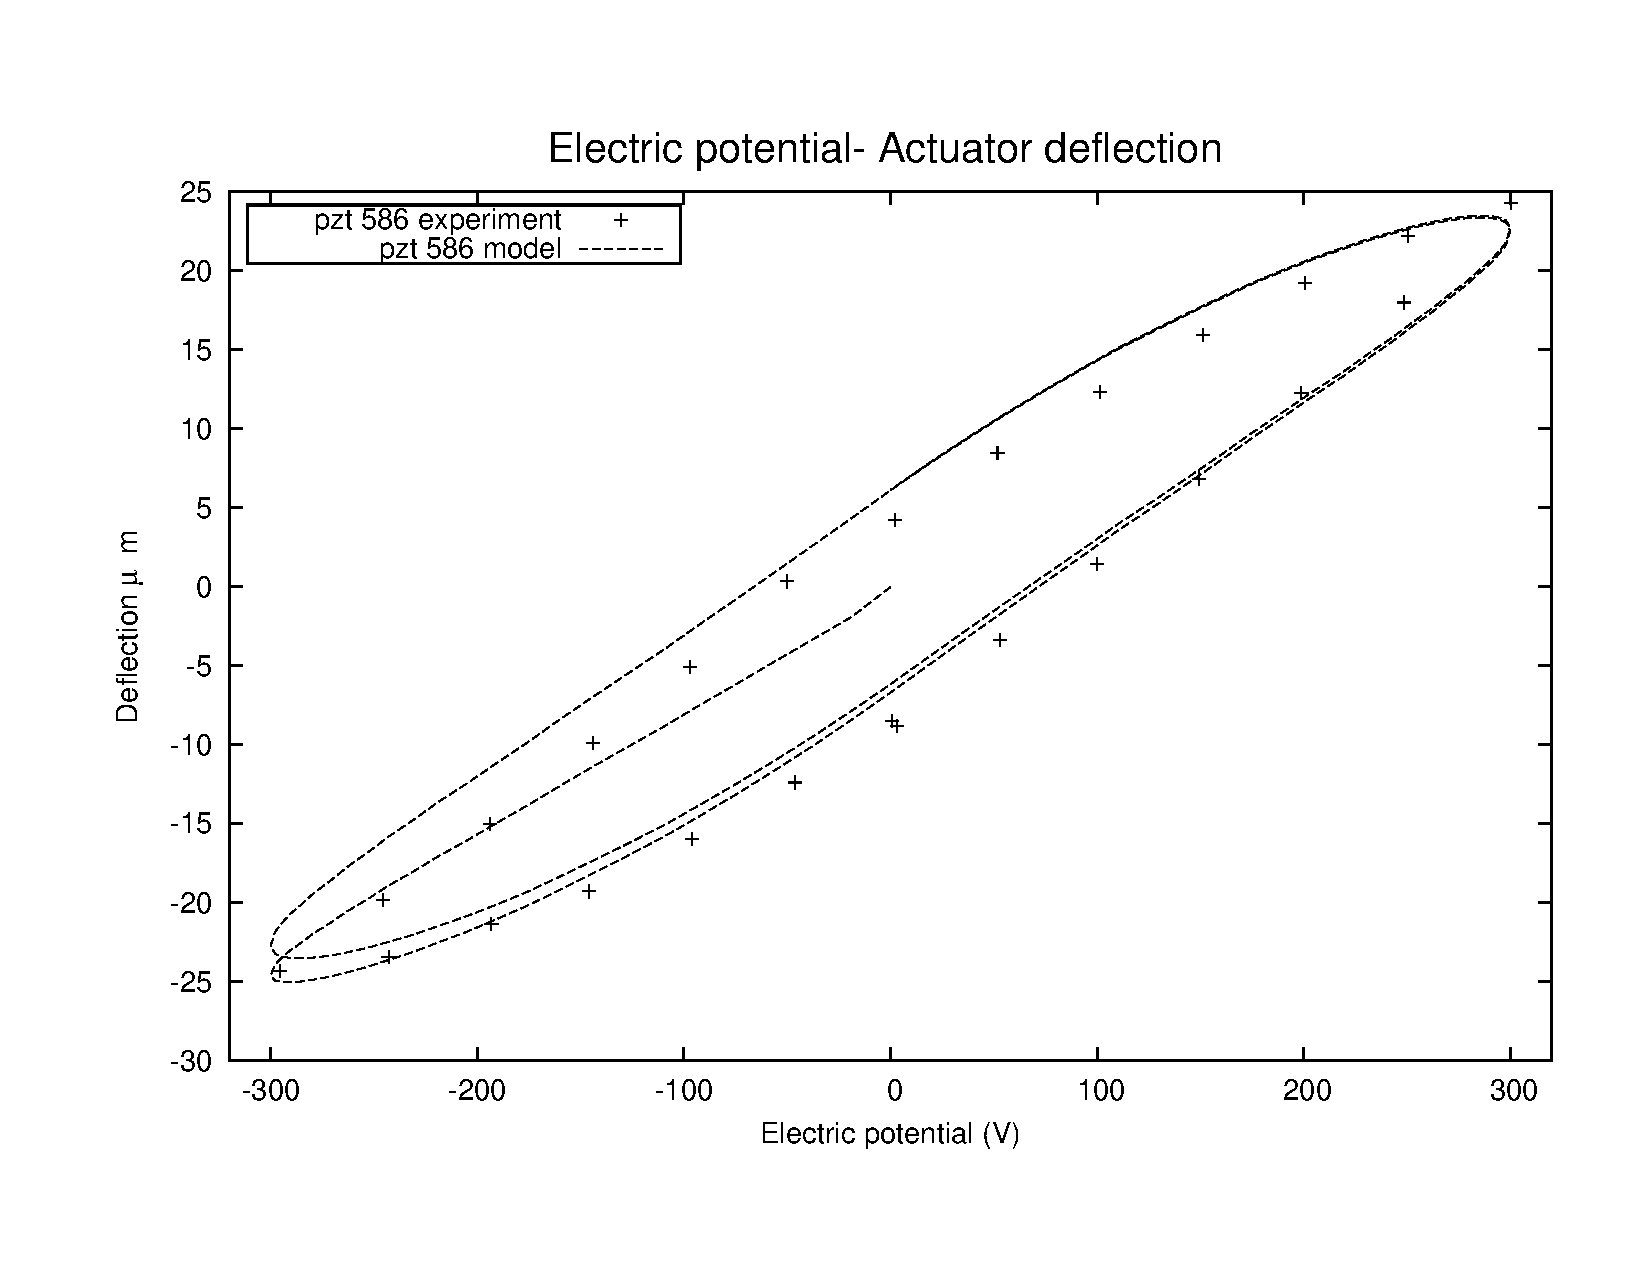
\includegraphics[width=5.0in]{./chap_3_minor_loop/figures/result_pzt_586.pdf}
\caption{Tip deflection of PZT-586, comparing FEM model with experiment}
\label{fig:PZT_586_XP_Calib}
\end{figure}

The displacement due to this applied electric field is obtained from the FE simulation. 
The corresponding displacement contour at applied electric fields are shown in figure \ref{fig:PZT-586_response}. 
The comparison between the time-dependent hysteresis response from current simulation and experiment are shown in figure \ref{fig:PZT_586_XP_Calib}. 
The nonlinear hysteresis response is captured effectively by taking the electro-mechanical coupling coefficients to be a nonlinear function of applied electric field. 
The material data are calibrated to fit the experimental data presented in \cite{Alexander,Alexander2003}. 
The rest of electro-mechanical properties are taken to be same as PZT and presented in table \ref{table:MatPZT_PZT_586}. 
The nonlinear coefficients are defined with respect to the applied electric field in the radial direction.
\begin{table}
\caption{Material properties of PZT-586 actuator \cite{Alexander}}
\centering
\begin{tabular}{c c c} \hline
Young's Modulus&62& $GPa$\\ \hline
Poisson's Ratio&0.3& \\  
$e_{212}$ &-32.51&$C/m^2$\\ 
$e_{122}$ &13.77&$C/m^2$\\ 
$e_{111}$ & -16.92&$C/m^2$\\ 
$\kappa_{11}=\kappa_{22}$ & 4 &pF/m\\ 
$\kappa_{33}$ & 2 &pF/m\\ 
$\widehat{b}_{1122}$ & $3.35 \times 10^{-5}$ &  $ N/V^2 $\\ 
$\widehat{b}_{1111} $ & $-3.35 \times 10^{-5}$ &$ N/V^2 $\\ 
$\kappa_{11}=\kappa_{22}$ & 4 &pF/m\\ 
$\kappa_{33}$ & 2 &pF/m\\ 
${}^{0}K_{ijk}^{e}$&1.0&\\ 
${}^{1}K_{ijk}^{e}$&-0.4&\\ 
${}^{0}\lambda_{ijk}^{e}$&0&\\ 
${}^{1}\lambda_{ijk}^{e}$&0.5&\\ \hline 
\end{tabular}
\label{table:MatPZT_PZT_586}
\end{table}
Another actuator, MSI-53, is considered in order to examine performance of FE model. 
The geometry of this actuator is shown in figure \ref{fig:MSI_53_Geometry}. 
The distribution of electric potential in the actuator is shown in figure \ref{fig:MSI_53_XP_contour}. 
The material properties of MSI-53 that are used for the FE analysis are given in table \ref{table:MatPZT_MSI_53}. 
It is noted that frequency of applied electric field is taken to be 0.1Hz. 
\begin{table}
\caption{Material properties of MSI-53 actuator \cite{Alexander}}
\centering
\begin{tabular}{ c c c } \hline
Young's Modulus&60.06&$GPa$\\ \hline
Poisson's Ratio&$0.3$&\\ 
$e_{111}$ &-20.92&$C/m^2$\\
$e_{122}$ &17.06&$C/m^2$\\
$e_{212}$ &-45.74&$C/m^2$\\
$\kappa_{11}=\kappa_{22}$ & 4 & pF/m\\
$\kappa_{33}$ & 2 & pF/m \\
$\widehat{b}_{1122} $ & $3.35 \times 10^{-5}$ &  $N/V^2$ \\
$\widehat{b}_{1111} $ & $-3.35 \times 10^{-5}$ & $N/V^2$ \\
$\kappa_{11}=\kappa_{22}$ & 4 & pF/m \\
$\kappa_{33}$ & 2 & pF/m \\
${}^{0}K_{ijk}^{e}$&1.0&\\
${}^{1}K_{ijk}^{e}$&-0.4&\\
${}^{0}\lambda_{ijk}^{e}$&0&\\
${}^{1}\lambda_{ijk}^{e}$&0.5&\\ \hline 
\end{tabular}
\label{table:MatPZT_MSI_53} 
\end{table}
The nonlinear coefficients are defined with respect to the applied electric field in the radial direction.
The distribution of the axial displacement and electric field distribution for this actuator is shown in figure \ref{fig:MSI_53_XP_results}. 
The tip deflection response of this actuator is simulated using the presented electro-mechanical model and it is compared with experimental result shown in figure \ref{fig:MSI_53_XP_results}. 
There is a good agreement between experiment and the model. 
The nonlinear coefficient have a very small effect on the result, which could be due to a small amplitude of the electric field applied.

\begin{figure}
\centering
\includegraphics[width=3.0in]{./chap_3_minor_loop/figures/MSI_53_XP_Geometry-eps-converted-to.pdf}
\caption{Geometry of MSI-53 (dimensions are in mm)}
\label{fig:MSI_53_Geometry}
\end{figure}


\begin{figure}
\centering
\includegraphics[width=5.0in]{./chap_3_minor_loop/figures/telescopic_actuator_msi_53_elec_pot_deflection_uy-eps-converted-to.pdf}
\caption{Electric potential and deflection contour of MSI-53 Telescopic Actuator}   
\label{fig:MSI_53_XP_contour}  
\end{figure}
 

\begin{figure}
\centering
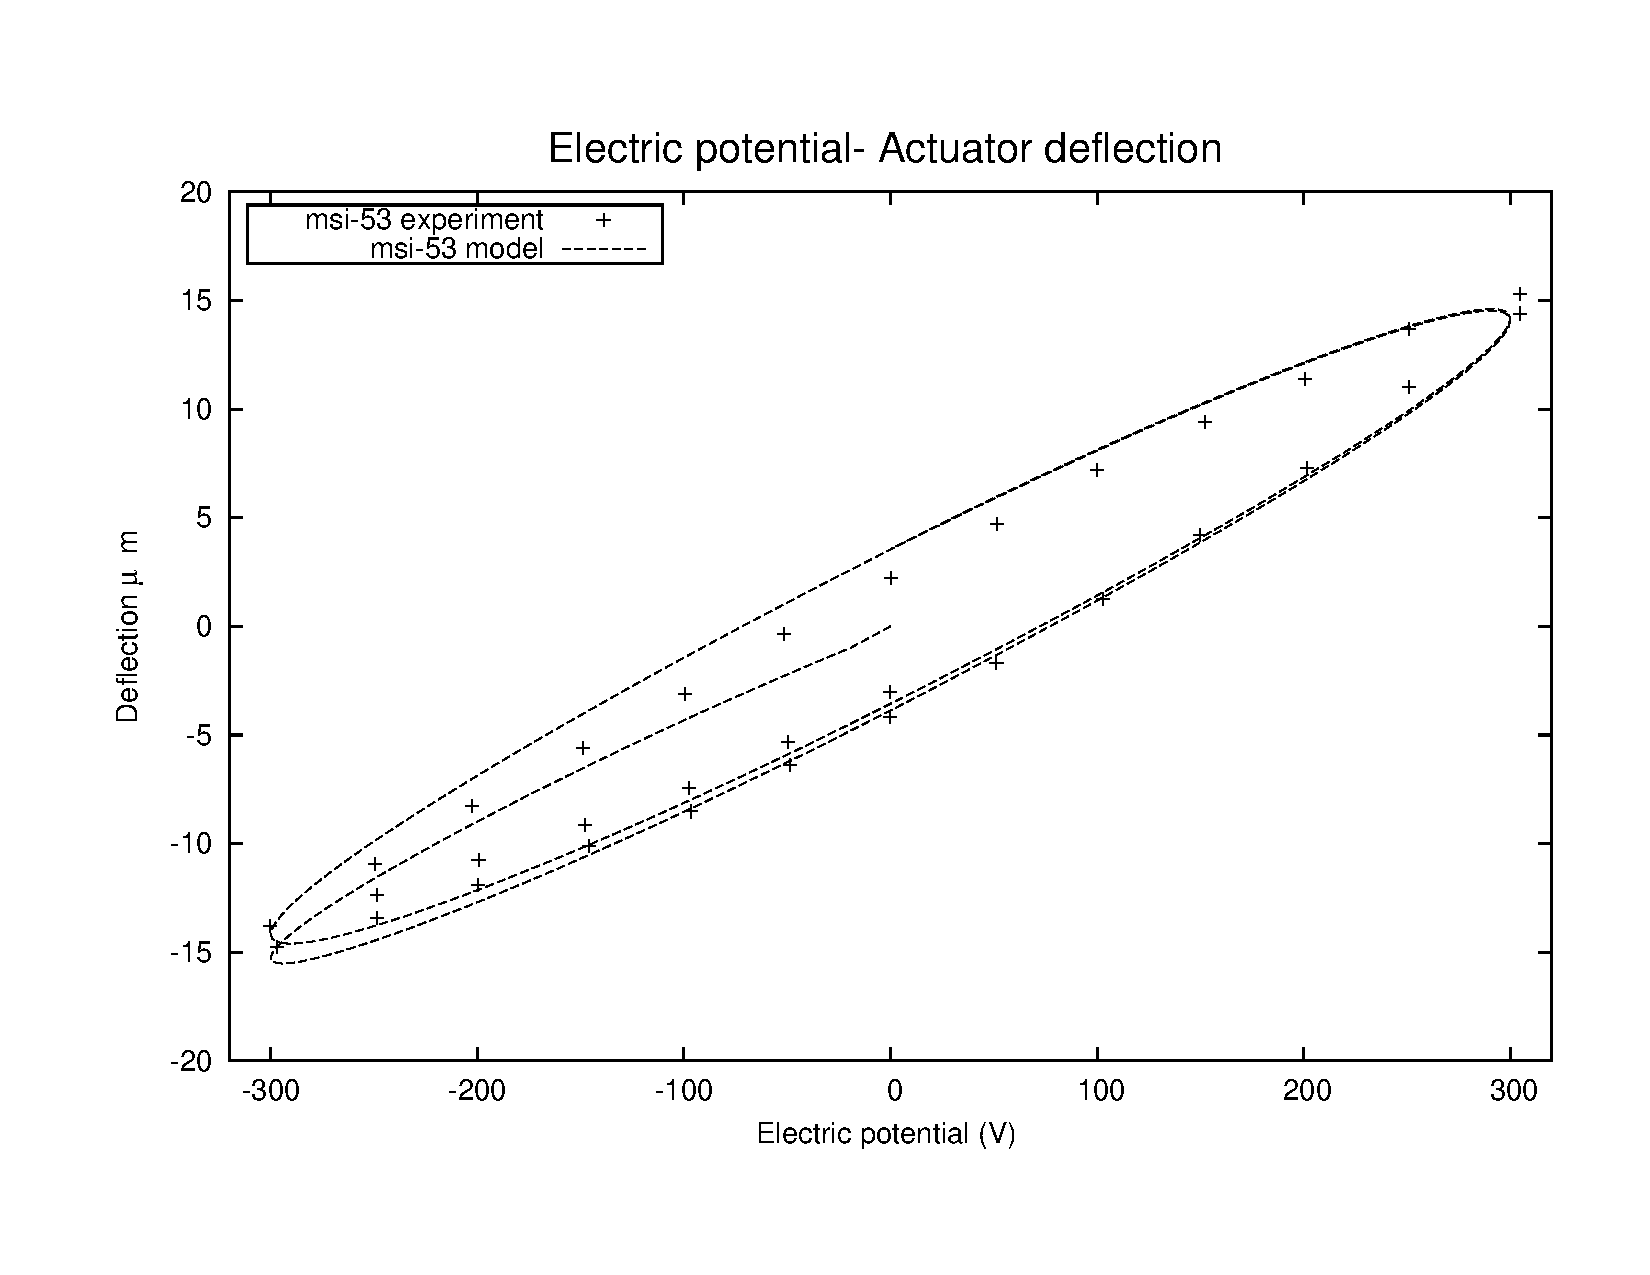
\includegraphics[width=5.0in]{./chap_3_minor_loop/figures/result_msi-53.pdf}
\caption{Tip deflection of MSI-53 comparing FEM model with experiment}
\label{fig:MSI_53_XP_results}
\end{figure}

